%\documentclass[12pt]{article}
\documentclass[12pt]{revtex4}
%\usepackage{graphics}
\usepackage[dvipdf]{graphicx}
%\usepackage{subfig}  % For subfloats
\usepackage{color}
\usepackage{multirow}
%\usepackage{subfig}  % For subfloats
\usepackage{subfigure}  % For subfloats
\usepackage{color}
\usepackage{multirow}
\usepackage{epsfig}
\usepackage{wrapfig}
\usepackage{rotating}
\usepackage{amsmath}
\usepackage{footmisc}
%\usepackage{subfigure}
\usepackage{hyperref}
%\usepackage[]{authblk}
\newcommand{\JLAB}{Thomas Jefferson National Accelerator Facility, Newport News, Virginia 23606}
\newcommand{\JP}{J/$\Psi~$}
\newcommand{\ee}{$e^+e^-~$}
\newcommand{\mumu}{$\mu^+\mu^-~$}


\begin{document}

\title{Possibilities of pentaquark search with CLAS12}
\author{M. Battaglieri, V. Burkert, A. Celentano, R. De Vita, V. Kubarovsky, P. Nadel-Turonski, R. Paremuzyan, S. Stepanyan}
%\affiliation{\JLAB}
\date{\today}

\begin{abstract}
\vspace{1.cm}

The hidden charmed pentaquark states claimed by LHCb, $P_c(4380)$ and $P_c(4450)$, can be searched/studied using CLAS12 and the 11 GeV electron beams. There are already two approved experiments, E12-11-005 and E12-12-001, that can search for these states within their proposed run conditions in near-to-real photoproduction. There is also a proposal for studying time-like photon and vector meson electroproduction, which can be suitable for pentaquark search in electroproduction. These experiments are complimentary, they will study the same reaction in different final states and kinematics. In this note description of different options for pentaquark studies using the CLAS12 detector is presented with mass resolution and the statistical reach of each experiment.
%a approved in the same reaction as the Time-like Compton Scattering and J/$\Psi$ photoproduction in the experiment E12-12-001. In this note the kinematics, detector performance, and possible options for the charmed pentaquark search is described. Response of the CLAS12 is simulated using Fast-MC.     
\end{abstract}

\maketitle


\section{Introduction}

LHCb recently announced the 
discovery of two exotic structures in the $J/\psi + p$ decay channel, which have been referred to as charmonium-pentaquark states $P_c(4380)$ and $P_c(4450)$, and claimed that the minimum quark content is $c\bar c u u d$~\cite{lhcb_penta}. The pentaquarks were observed in the decay $\Lambda_b^0\to K^-P_c^+$, $P_c^+\to J/\psi p$.
The decays of conventional baryons to $J/\psi+X$ are strongly suppressed by OZI rule and hence  these resonances should contain a $c\bar c$ pair  and  3 light quarks in the initial state.
%In addition, the masses of these states ($\approx$~4.4 GeV) are close to the sum of the $J/\psi$ and proton masses. The narrow width (especially for the $P_c(4450)$) supports the hypothesis that these heavy baryonic states have small probability to decay to the low mass mesons and baryon, which would be very difficult to explain if these states consist of the light quarks only. 
So the interpretation of these structures as pentaquark with hidden charm looks very reasonable. 

Clearly, understanding of the nature of the discovered hidden-charm pentaquark states, and possibly searching for similar states with other quantum numbers, requires further experimental studies. 
These states were observed in the decay mode $J/\psi+p$. For this reason it is natural to expect that these states can be produced in photoproduction process $\gamma+p\to P_c\to J/\psi+p$ where these states will appear as s-channel resonances at photon energy around 10\,GeV. 

The CLAS12 experiments, E12-11-005 and E12-12-001 \cite{e1211005, e1212001} will study photoproduction of J/$\Psi$ in electron scattering experiment on hydrogen using the $11$ GeV electron beam. The reaction $e p\to e^\prime p \gamma^* \to e^\prime p l^+ l^- $, where $\gamma^*$ either a timelike photon or a vector meson, can be studied for decay leptons ($l$ is $\mu$ or $e$) invariant masses up $3.4$ GeV for the total-of-center mass energies up to $\sqrt{s}=4.64$ GeV.    
In this note, options for studying charmed pentaquarks using CLAS12 is presented. Brief description of each experiment is given with the key kinematic and experimental parameters such as acceptances and resolutions. Options for improvements of the statistical reach of these experiments are discussed as well. Some of the presented material is a repetition of what has been presented in the experiment proposals, some additional plots are shown for proton-J/$\Psi$ system.

\section{Photoproduction cross section}

There have been already several articles on the arxiv that give estimates for photoproduction cross section of $P_c(4380)$ and $P_c(4450)$ \cite{pt1, pt2, pt3}. The production of pentaquarks proceeds as an $s$-channel resonance in the (pJ/$\Psi$) system. First photon converted to vector meson, J/$\Psi$, which later is absorbed by the proton as shown in Fig.\ref{fig:fndiag} \cite{pt4}.

\begin{figure}[ht]
\begin{center}
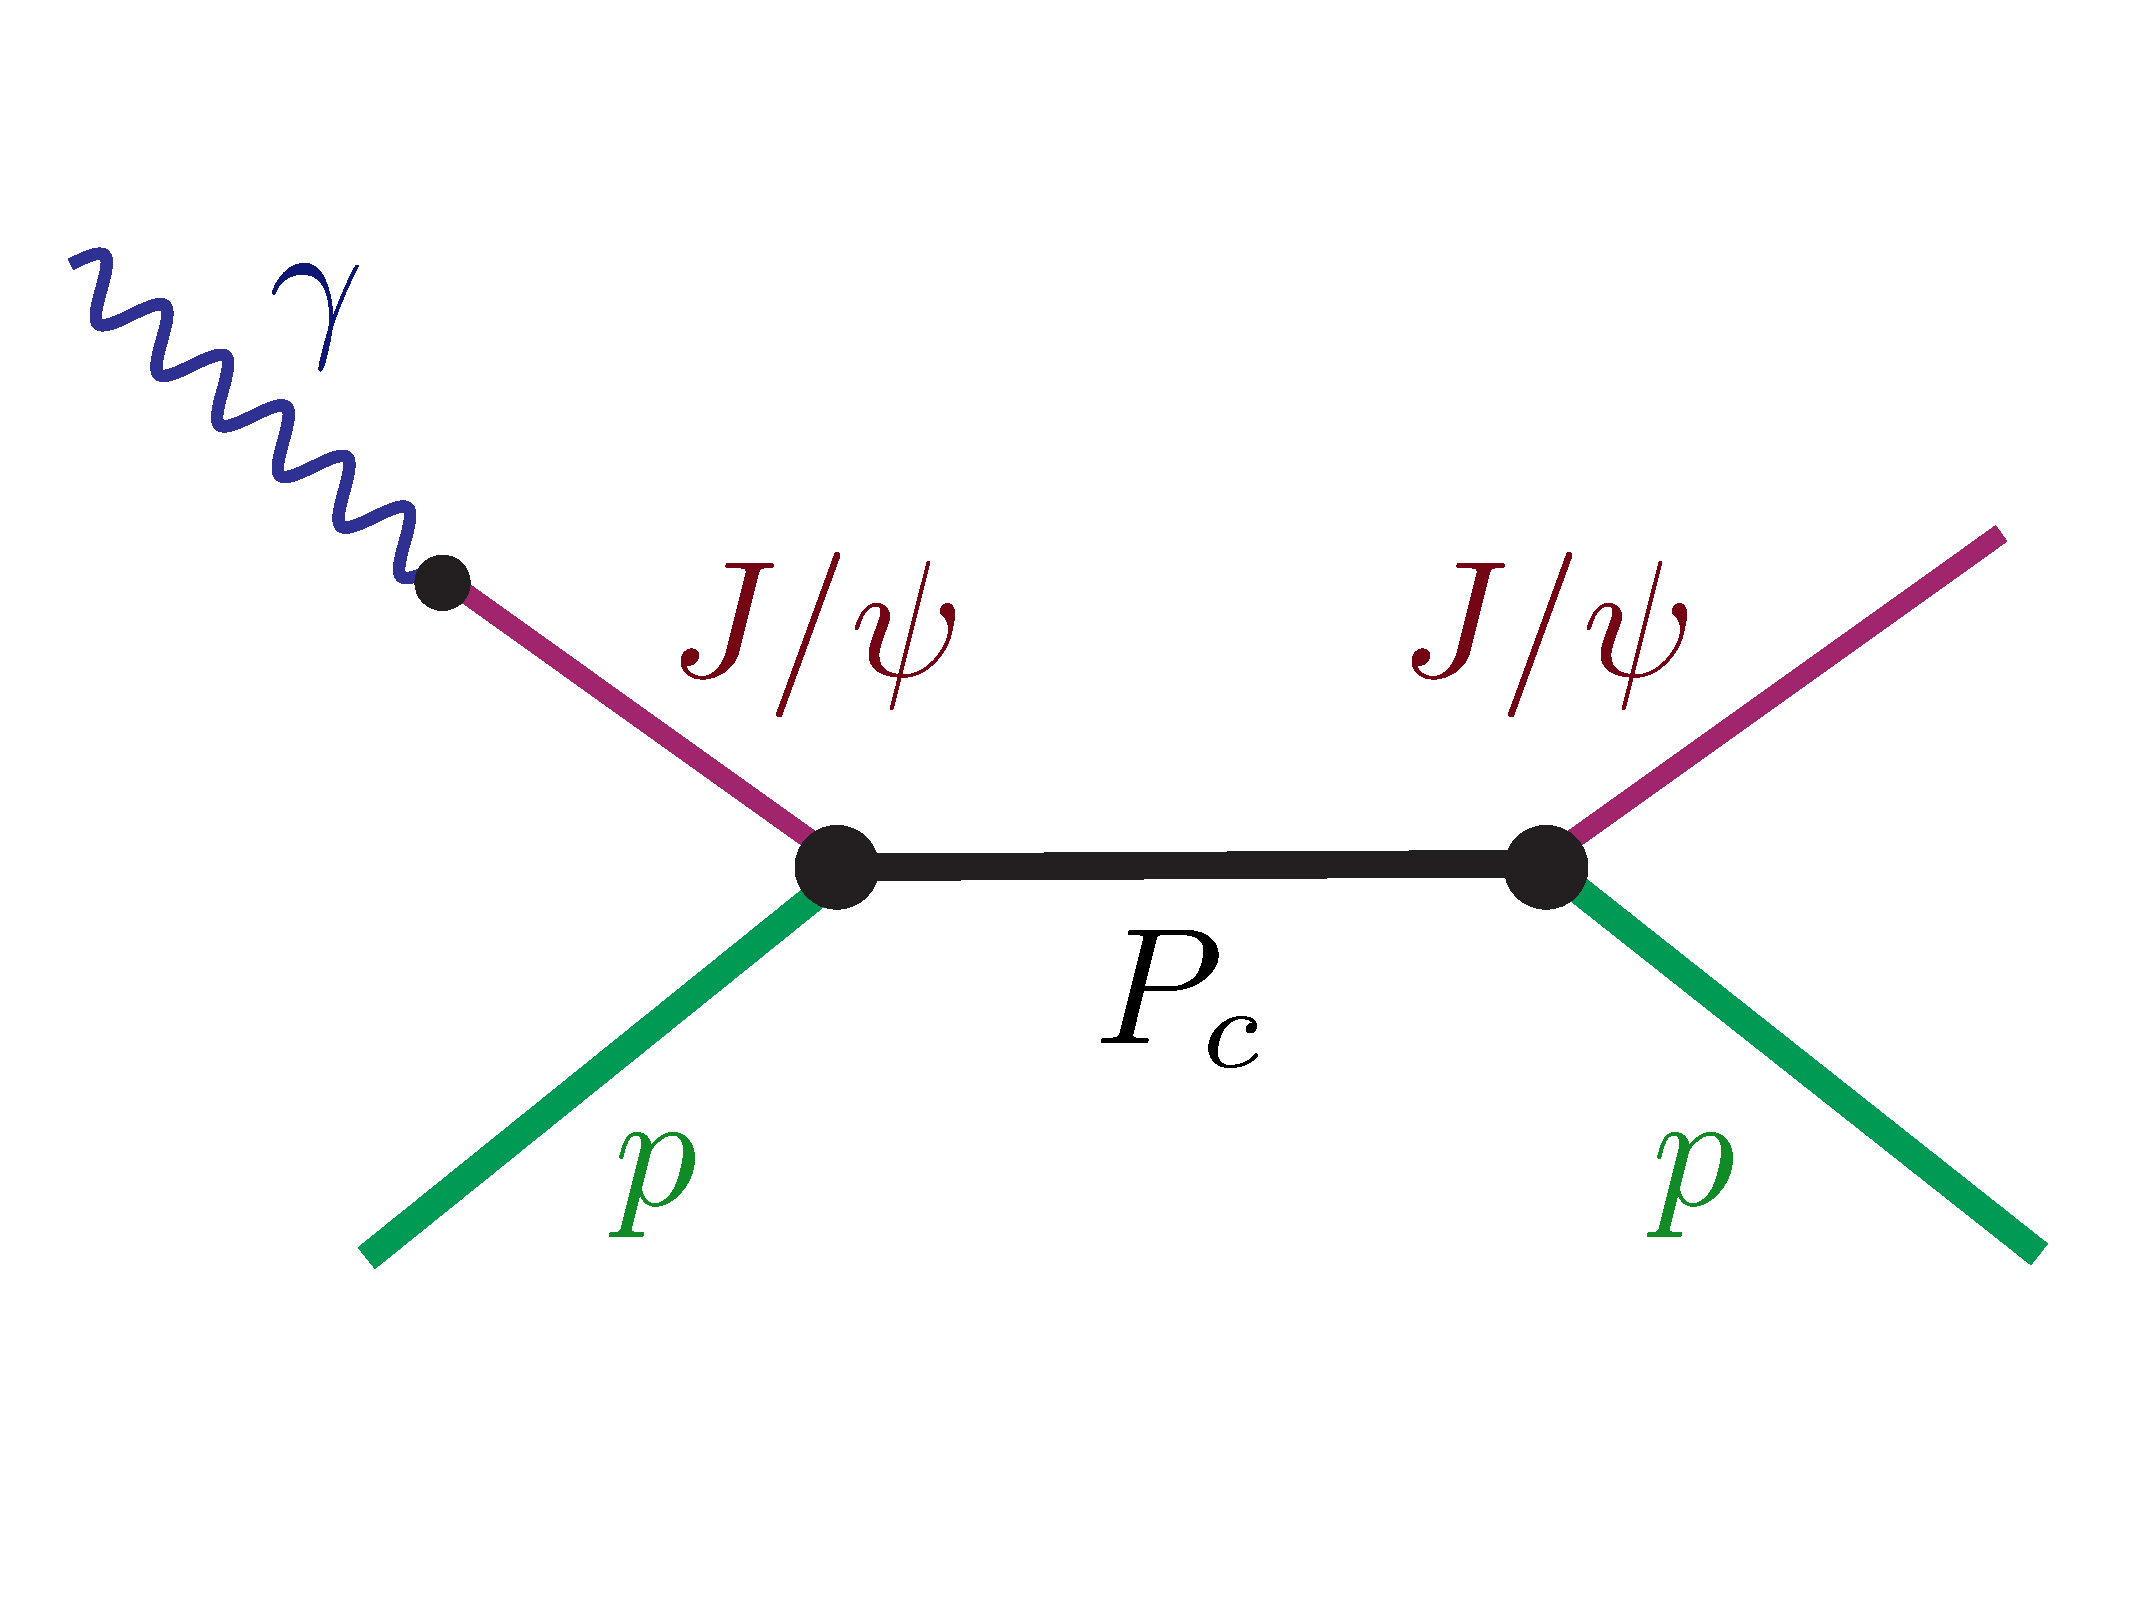
\includegraphics[width=0.45\textwidth]{Jipsi5.pdf}
\caption{Feynman diagram for the pentaquark photoproduction process.}    
\label{fig:fndiag}
\end{center}
\end{figure} 

For a resonance $P_c$ in the $s$ channel the photoproduction cross section of the reaction 
$\sigma(\gamma + p \to P_c \to J/\psi + p)$
is given by the standard Breit-Wigner expression (see e.g. in Ref.~\cite{pdg}, Sec.~48.1.)
\begin{equation}
\sigma(W) = { 2 J +1 \over 4} \, {4 \pi \over k^2} \, {\Gamma^2/4 \over (W-M_c)^2 + \Gamma^2/4} \, Br(P_c \to \gamma + p) \, Br(P_c \to J/\psi +p)~,
\label{bw}
\end{equation}
where $J$ is the spin of the $P_c$ resonance, $W=\sqrt{s}$  is the c.m. energy,  $M_c$ is the resonance mass, $\Gamma$ is the total width and $k$ is the center of mass (c.m.) momentum of the colliding particles. At the resonance mass peak this expression gives numerically (at $k \approx 2.1\,GeV$)
\begin{equation}
\sigma_{max}\approx { 2 J +1 \over 4} \, Br(P_c \to \gamma + p) \, Br(P_c \to J/\psi +p) \, 1.1 \times 10^{-27} {\rm cm}^2~.
\label{bwm}
\end{equation}

It was shown in~\cite{pt2} that the bounds for the formation cross section at the resonance maximum were give as:
\begin{eqnarray}
&& 1.5 \times 10^{-30}\, {\rm cm^2} \, < \, {\sigma_{max}[\gamma + p \to P_c(4380) \to J/\psi + p] \over Br^2[ P_c(4380) \to J/\psi+p]} \, < \, 47 \times 10^{-30} \, {\rm cm^2}~, \nonumber \\
&& 1.2 \times 10^{-29}\, {\rm cm^2} \, < \, {\sigma_{max}[\gamma + p \to P_c(4450) \to J/\psi + p] \over Br^2 [ P_c(4450) \to J/\psi+p]} \, < \, 36 \times 10^{-29} \, {\rm cm^2}~,
\label{modn}
\end{eqnarray}
The expected total cross section for J/$\Psi$ photoproduction at the pentaquark peak is $\sim 0.1\times 10^{-33}$ cm$^2$.  

\section{Experiment E12-12-001}

E12-12-001 \cite{e1212001} will study Time-like Compton Scattering (TCS) and photoproduction of J/$\Psi$ near threshold in the reaction $e p\to p \gamma^* (e^\prime )\to  p e^+ e^- (e^\prime)$. Three particles will be detected in final state, recoil proton, and the $e^+$ and $e^-$ from the time-like (virtual) photon or vector meson decays. The scattered electron ($e^\prime$) will be identified in the missing momentum analysis. Requiring for the missing momentum to be in the direction of the beam, $\theta_x\sim0$, and the missing mass to be $m_x\simeq 0$, one effectively selects events from the quasi-real phtoproduction of electron pairs off hydrogen. This technique has been successfully used for analysis of CLAS 6 GeV electroproduction data and has been proven to be excellent way to study photoproduction reactions when all hadronic final state particles are detected, see  \cite{tcs_rafo, jpc_prop}. 
%The first such analysis was done using the CLAS e1-6 data set where in the triggered events that did not contain an electron in the reconstructed final state (due to very loose electron trigger definition) four photons and a proton were found. Further analysis of such events showed that the most of these events are p$\pi^0\pi^0$ and p$\pi^0\eta$ final states in the reaction $ep\to p\gamma\gamma\gamma\gamma X$, with missing particle $X$ being an electron ($m_x\simeq 0$) with momentum in the direction of the beam ($\theta_x\sim0$), see for example \cite{jpc_prop}. The second analysis TCS analysis from the CLAS $6$ GeV electroproduction data (CLAS e1-6 and e1f runs)  \cite{tcs_rafo}. Similar analysis has been done for the photoproduction of p$\pi^0\pi^0$ and p$\pi^0\eta$ final states in the reaction $ep\to p\gamma\gamma\gamma\gamma X$ from the CLAS e1-6 data set, see for example \cite{jpc_prop}. 

The main goal of the J/$\Psi$ part of the E12-12-001 is to measured the total cross section near the threshold and study $t$-dependence that can shade light on nucleon gluonic form-factors. There are no published experimental data on J/$\Psi$ photoproduction below photon energies $\sim 11$ GeV. All published data above $12$ GeV suggest 2-gluon exchange mechanism for production, while on point from Crrnell and few unpublished loins from SLAC show enhancement of the cross section near the threshold that lead to suggestion then 3-gluon exchange may become dominant in that region \cite{bchl}, or it might be due to the resonance enhancement, see discussion below. Clearly, analyze of E12-12-001 will cover exactly the same final state in exactly the same energy range where aforementioned pentaquark states have been found and will be able to search for these states. Whiie E12-12-001 is part of the CLAS12 Run Group-I and will have constraints on running conditions from other experiments in the group, there is 20 days of dedicated time for E12-12-001 that can be used if drastic changes to the overall run conditions will be needed (e.g. making bigger Moller shield and run with x10 higher luminosity).

Below are some MC studies for J/$\Psi$ photoproduction near the threshold, covering the region of the  charmed pentaquarks.

\subsection{Kinematics} 

With beam energy of $11$ GeV, all three final state particles, a recoil proton, and the decay leptons from J/$\Psi$ photoproduction will be detected in CLAS12 Forward Detector (FD). In Fig. \ref{fig:kine}, scattering angle ($\theta$) is plotted agains particle momentum ($p$) for protons (top), and electrons and positrons (bottom) for quasi-real photoproduction of \JP in photon energy range from threshold to $11$ GeV. Kinematics of the reaction is simulated with expected $s$- and $t$-dependences of the cross section (see below). Protons are energetic and are produced in forward direction (due to high momentum transfer near the threshold). There are some electrons at large angles, $\theta>35^\circ$, however CLAS12 Central Detector (CD) is not suited for electron detection and identification, so we will consider detection of the final state particles only in CLAS12-FD.  

\begin{figure}[htbp]
\begin{center}
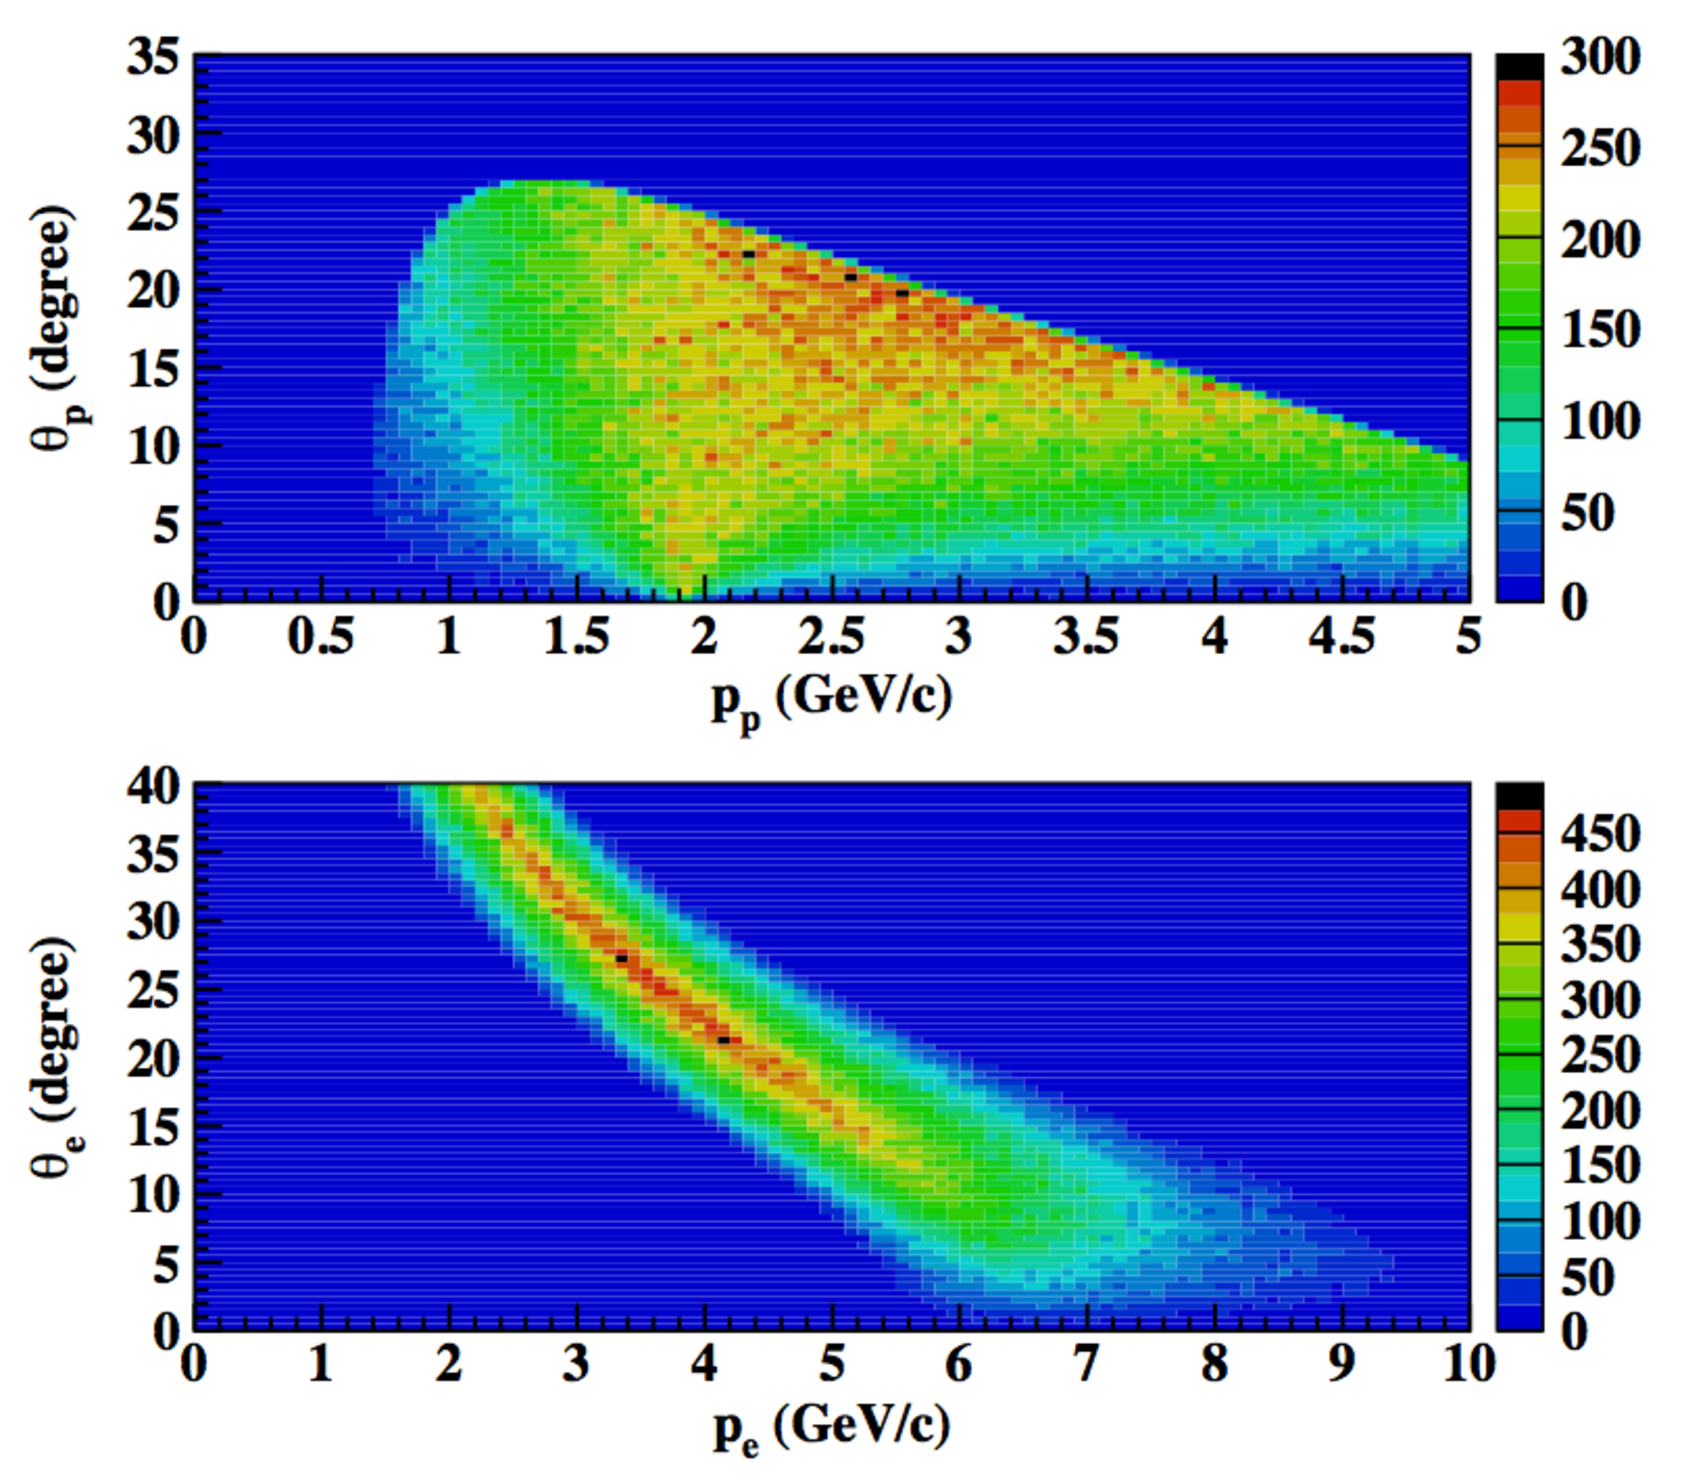
\includegraphics[width=0.8\textwidth]{p_theta_pe.pdf}
\caption{Scattering angle vs. momentum for protons (top) and electrons ($e^-$, $e^+$) (bottom) in the reaction $e p\to J/\Psi p (e^\prime)$ for quasi-real photon energies from the threshold to 11 GeV.}
\label{fig:kine}
\end{center}
\end{figure}

With above consideration and using CLAS12 Fast-MC, the acceptance (efficiency) of detecting all three particles from hadronic final state will be about $10\%$ for the maximum torus field setting, see Fig. \ref{fig:accept}, and arises slowly with lowering the field. In Fig. \ref{fig:mpee}, the invariant mass distribution for the detected (p$e^+e^-$) system is presented. The charmed pentaquarks are in the center of the mass acceptance in the kinematics of the E12-12-001.  

\begin{figure}[htbp]
\begin{center}
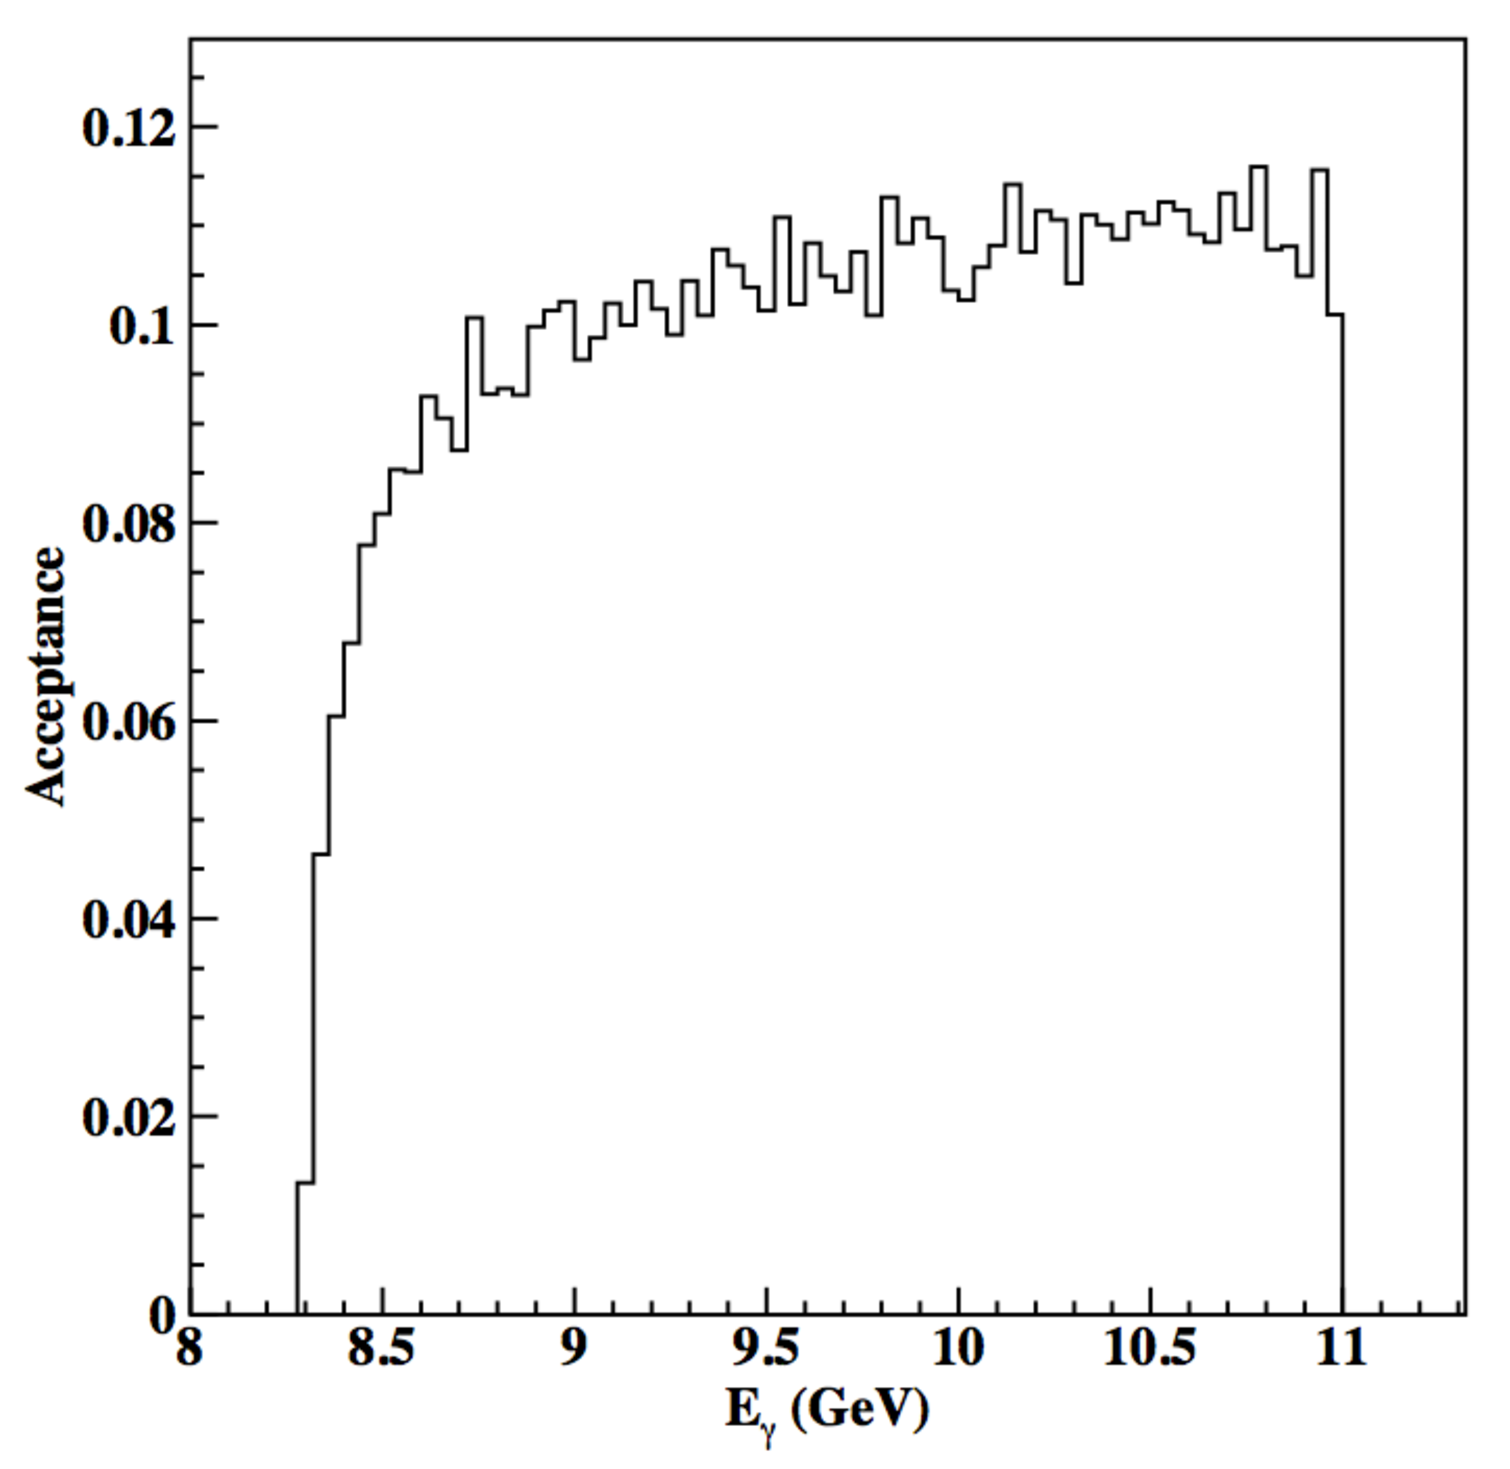
\includegraphics[width=0.5\textwidth]{acceptance_u.pdf}
\caption{Acceptance simulated using CLAS12 Fast-MC for (p$e^-e^+$) in the reaction $e p\to J/\Psi p (e^\prime)\to e^+ e^- p (e^\prime)$ for quasi-real photon energies from the threshold to 11 GeV.}
\label{fig:accept}
\end{center}
\end{figure}

\begin{figure}[htbp]
\begin{center}
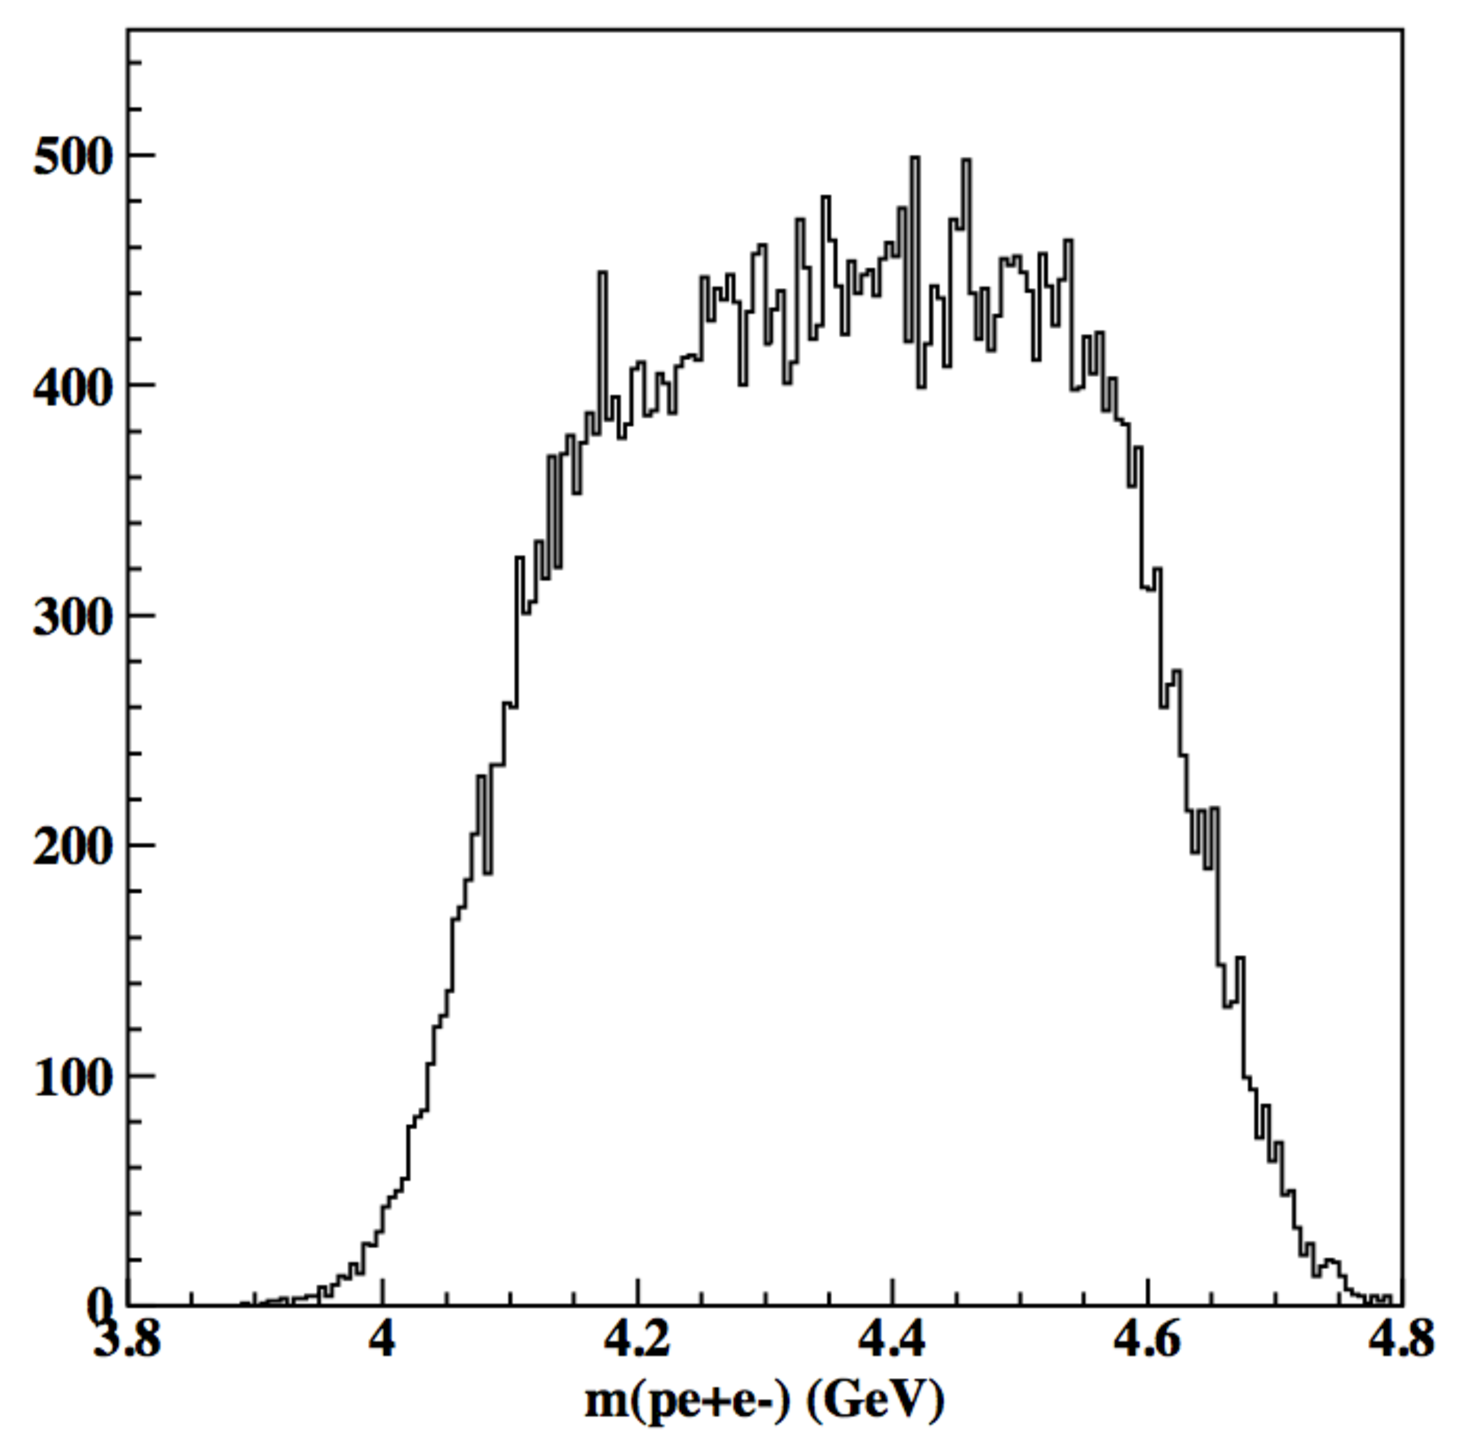
\includegraphics[width=0.5\textwidth]{m_pee.pdf}
\caption{Mass distribution of (p$e^-e^+$) in the reaction $e p\to J/\Psi p (e^\prime)\to e^+ e^- p (e^\prime)$ for quasi-real photon energies from the threshold to 11 GeV. The smeared in Fast-MC values of momenta and angles are used to calculate the invariant mass.}
\label{fig:mpee}
\end{center}
\end{figure}


\subsection{Mass resolutions} 

In order to search pentaquark states, especially narrow $P_c(4450)$, reasonably good mass resolution is required. In 2013, by request of the run group, studies have been conducted to see the effect of the torus field setting on different experiments. These studies were done to optimize acceptance and resolution. In relation to the \JP measurements, we studied the invariant mass resolution of $e^+e^-$. In Fig. \ref{fig:jp_mres} top, results of that studies are shown. Back then we concluded that lowering the field to $75\%$ of its nominal value or even to $60\%$ should not harm the \JP measurements.
\begin{figure}[htbp]
\begin{center}
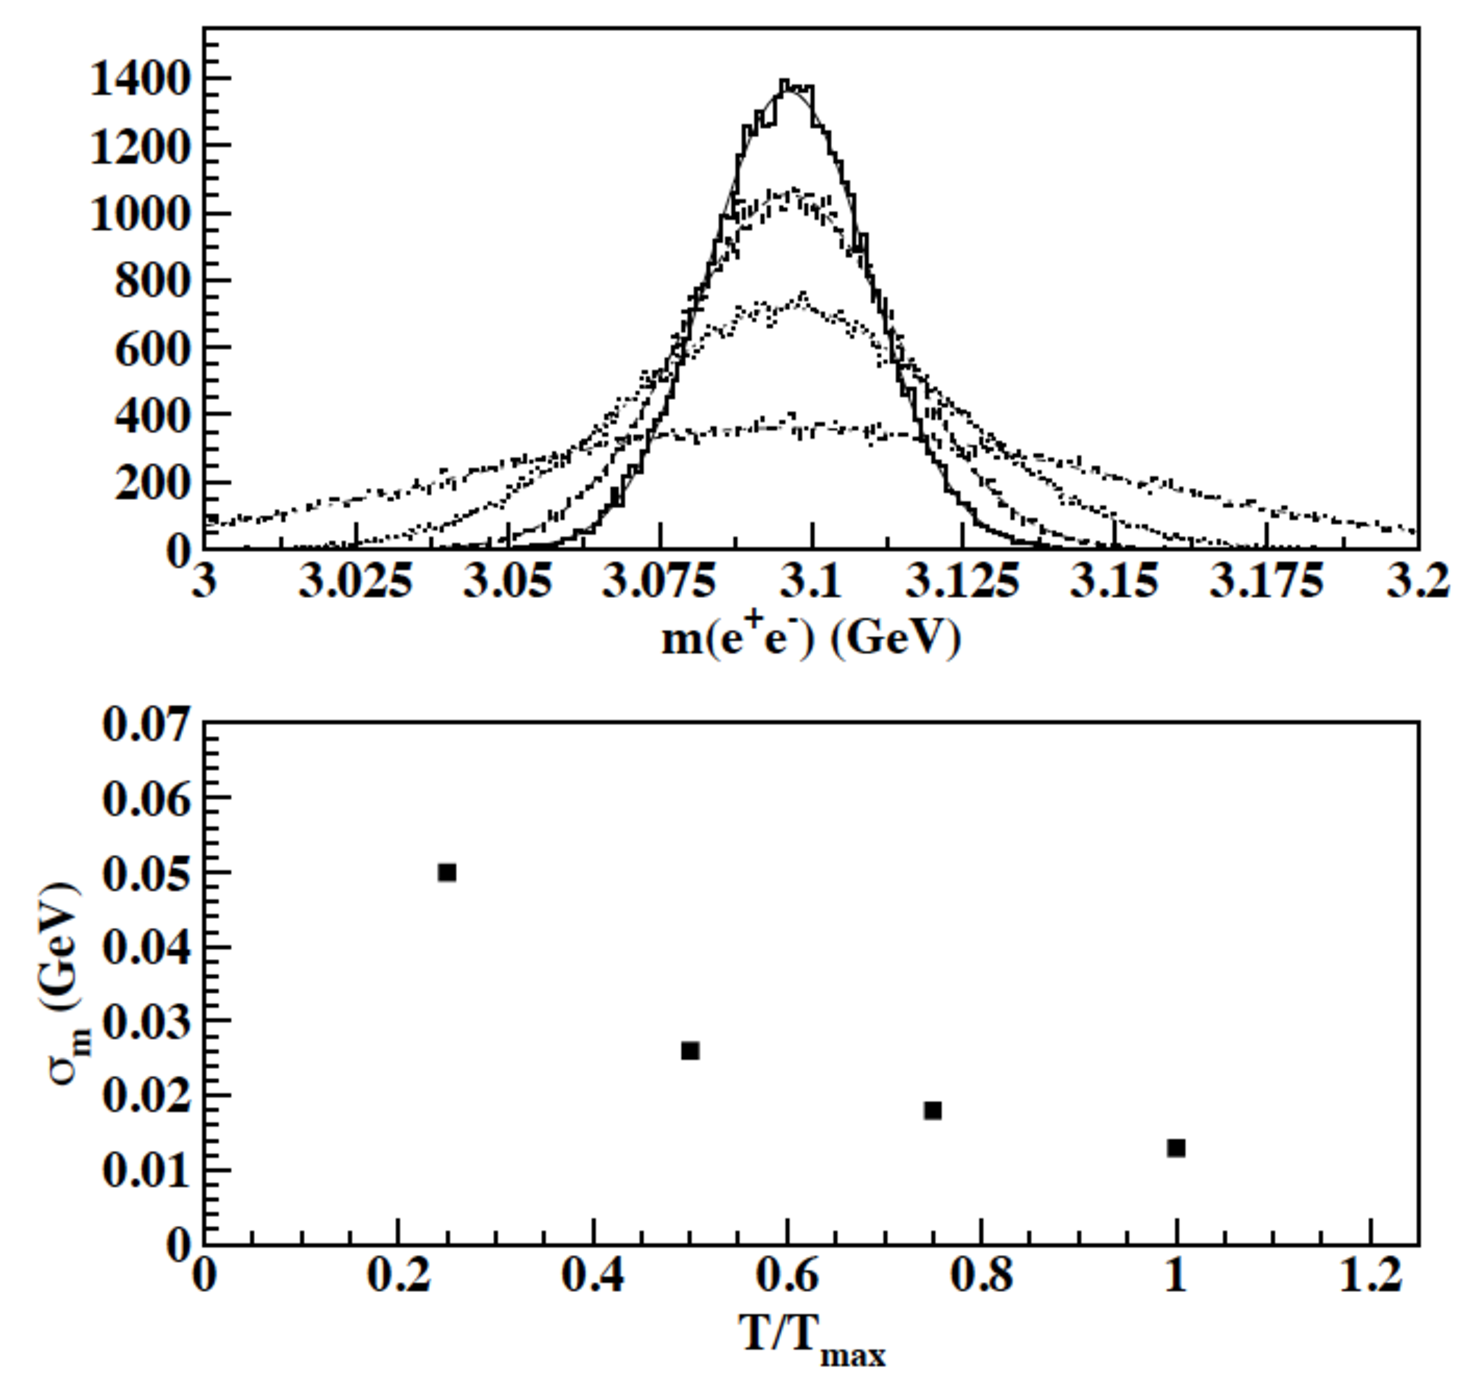
\includegraphics[width=0.7\textwidth]{jp_mass_res.pdf}
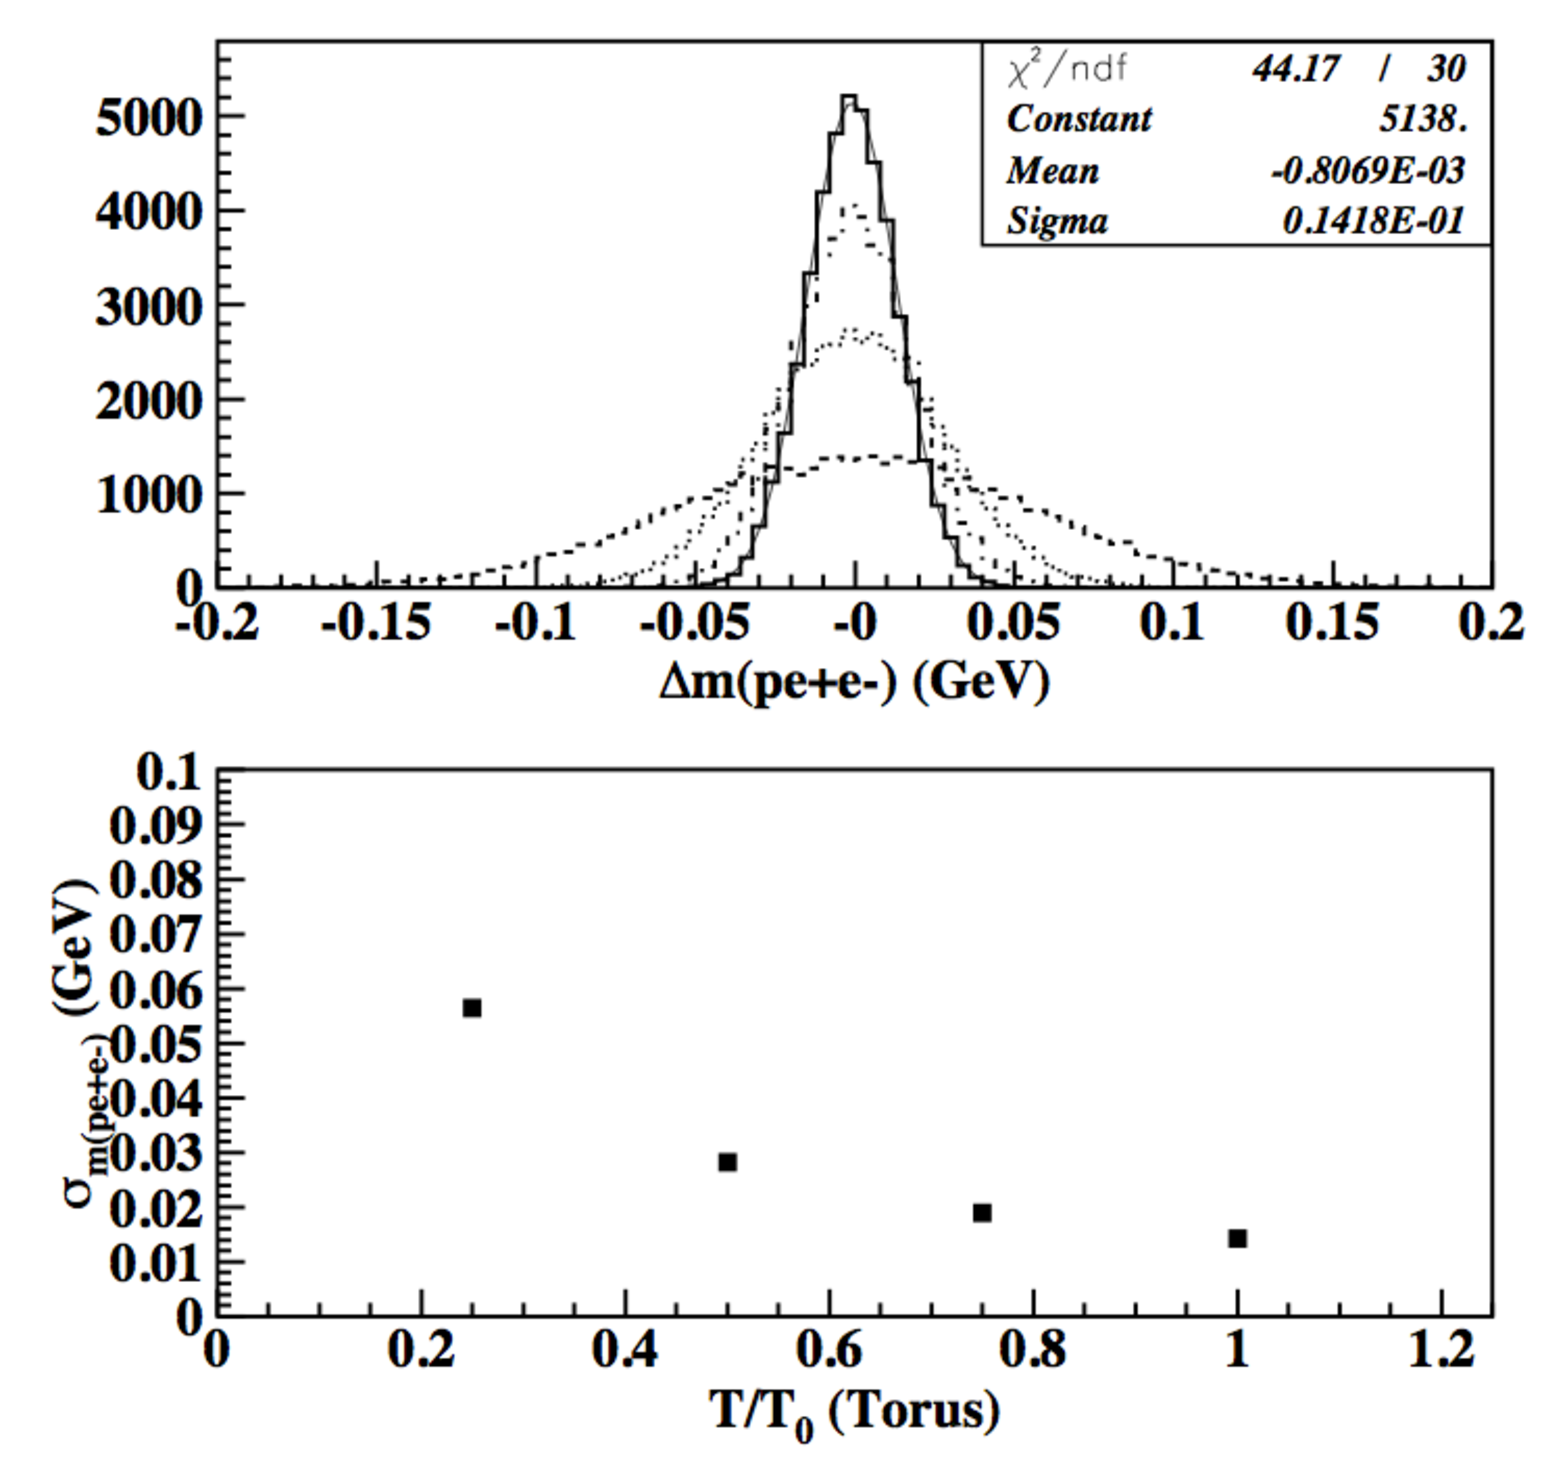
\includegraphics[width=0.7\textwidth]{pee_mass_res.pdf}
\caption{Invariant mass resolution for ($e^+e^-$) pair at J/$\Psi$ mass as function of CLAS12 torus field settings. Invariant mass resolution for (p$e^+e^-$), detected in CLAS12 FD, as function of CLAS12 torus field settings. The ($e^+e^-$) are from J/$\Psi$ decay. The CLAS12 Fast-MC is used for the estimate.}
\label{fig:jp_mres}
\end{center}
\end{figure}

The same simulations and the Fast-MC setup is used to asses the invariant mass resolution of the (p$e^+e^-$) system for different torus field settings. The results are shown in th bottom panel of Fig. \ref{fig:mres}. The narrowest charmed pentaquark, $P_c(4450)$, has width of $\sim 40$ MeV, and therefore in order to have at least $2\sigma$ of the width, the field setting (resolution) cannot be lower than the $75\%$ of expected nominal setting (or equivalent to that resolution).  

%\begin{figure}[htbp]
%\begin{center}
%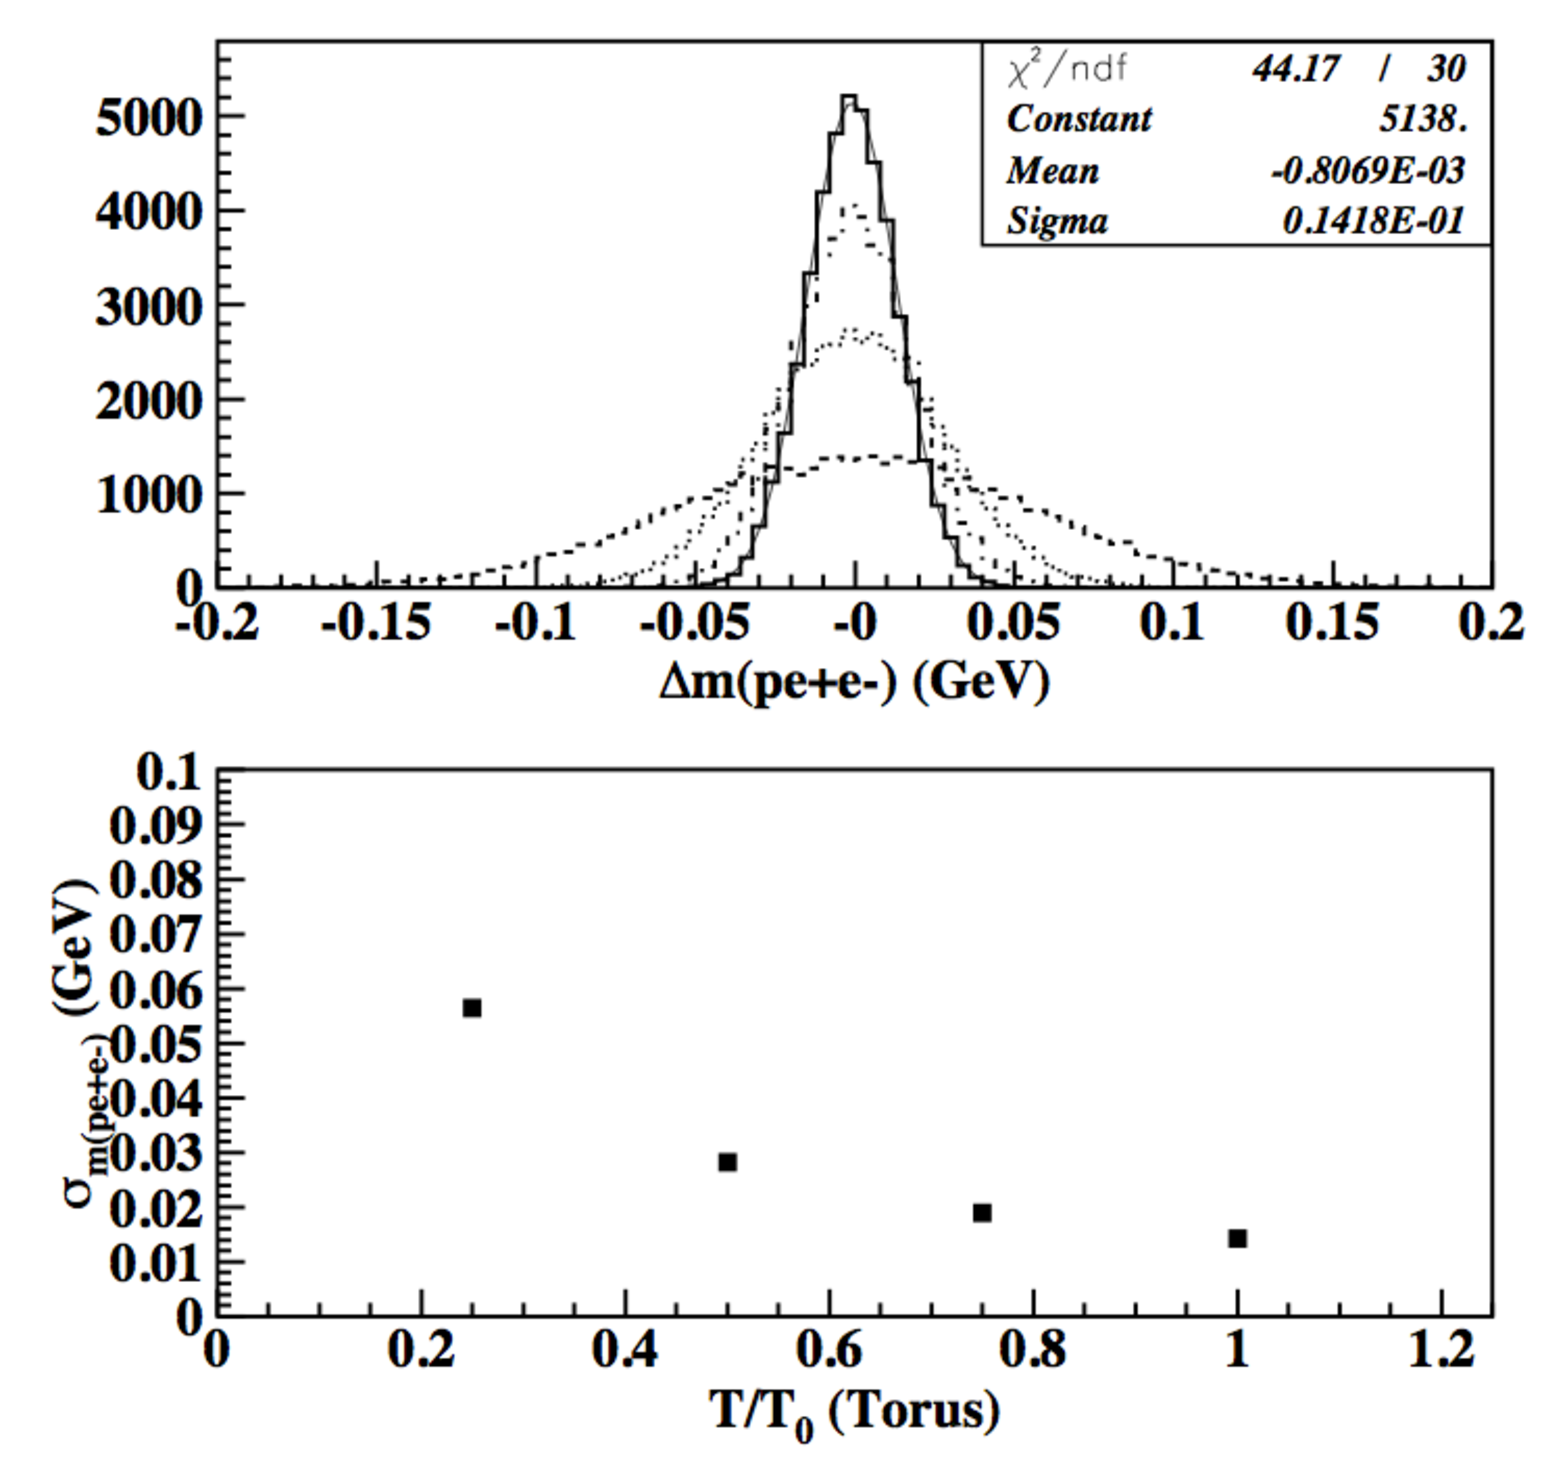
\includegraphics[width=0.6\textwidth]{pee_mass_res.pdf}
%\caption{Invariant mass resolution for (p$e^+e^-$), detected in CLAS12 FD, as function of CLAS12 torus field settings. The ($e^+e^-$) are from J/$\Psi$ decay. CLAS12 Fast-Montecarlo is used for the estimate.}
%\label{fig:pee_mres}
%\end{center}
%\end{figure}

\clearpage

\subsection{\JP cross section}

In the proposal E12-12-001 for the J/$\Psi$ rate estimate two models for photoproduction cross section from \cite{bchl} were studied.  The J/$\Psi$ photoproduction differential cross section was parametrized as (similar to but somewhat different from \cite{bchl}):
\begin{eqnarray*}
{d\sigma\over{dt}} = \sigma_{norm}\cdot (1-x)^n\cdot e^{-bt}\cdot{(s-M_p^2)^2\over{m_{J/\Psi}^k}}
\end{eqnarray*}
where $\sigma_{norm}$ is the normalization to the measured cross section at $\sim 12$ GeV where two models intersect and is equal to $3.34923$ nb/GeV$^2$ and $3.481$ nb for 2- and 3-gluon exchanges, respectively. The $x=E_{thr}/E_\gamma$ with $E_{thr}=8.2$ GeV, the slope $b=1.13$ GeV$^{-2}$ extracted from the available data, $s$ is the total center mass energy squared, and $M_p$ and $M_{J/\Psi}$ are the rest masses of the proton and J/$\Psi$ meson, respectively. The power parameters for 2-gluon exchange model are $n=2$ and $k=2$, and $n=0$ and $k=4$ for the 3-gluon exchange. A conservative assumption for the cross section via 2-gluon exchange was used  for the final rate estimates, red dashed line in Fig. \ref{fig:jpmeas}.

\begin{figure}[htbp]
\begin{center}
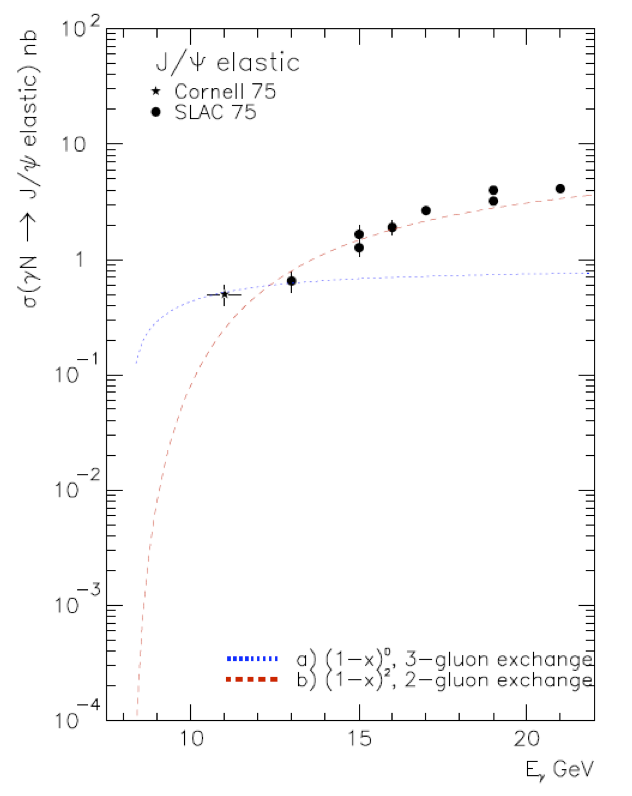
\includegraphics[width=0.7\textwidth]{jp_measured.pdf}
\caption{Existing data for the total cross section of the J/$\Psi$ photoproduction with predictions of possible behavior towards the threshold.}
\label{fig:jpmeas}
\end{center}
\end{figure}

\subsection{Photon flux}

In the electroproduction when the virtuality of the transferred photon is small $Q^{2} \sim 0$,  
 the electroproduction cross-section can be parametrized as a product of the photoproduction cross-section and the
 virtual photon flux.
 \begin{equation}
  \sigma_{e} = N_{\gamma}(E_{\gamma})\sigma_{\gamma}
 \end{equation}
 where $\sigma_{e}$ is the electroproduction cross-section, $\sigma_{\gamma}$ is
 the photoproduction cross-section, and the $N_{\gamma}(E_{\gamma})$ is a flux of virtual photon, that represents
 number of virtual photons in the unit range of photon energy. This is known as
 Equivalent Photon Approximation (EPA).
 
 In the electroproduction experiments, beam electrons will produce Bremsstrahlung photons in the target also,
 the flux of that photons is proportional to the target length.
 When the target length is not very small (w.r.t radiation  length of the target), then real photon flux
 can be significant and one needs to consider that also.
 
 The effective flux of photns therefore will be the sum of quasi-real (Virtual photon) and real
 (Bremsstrahlung) photon fluxes.
 
 The virtual photon flux is calculated using the following
 equation \cite{Phot_Flux1}
 \begin{equation}
  \Gamma(E_{\gamma}) = \frac{1}{E_{b}} \frac{\alpha}{\pi\cdot x}
  \cdot\left( (1 - x + \frac{x^{2}}{2})\cdot log(\frac{Q^{2}_{max}}{Q^{2}_{min}}) - (1 - x)\right)
 % (1/Eb)*\alpha/(PI*x)*( (1 - x + x*x/2)*log(\frac{Q2_{max}}{Q2_{min}}) - (1 - x));
 \end{equation}
where $E_{b}$ is the beam energy, $E_{\gamma}$ is the photon energy, $x = \dfrac{E_{\gamma}}{E_{b}}$, 
$Q^{2}_{min}$ is kinematically allowed minimum value of $Q^{2}_{min}$, and $Q^{2}_{max}$ is the
cutoff value on $Q^{2}$. 
 
 When electron passes a matter of the length $dx$, the number of Bremsstrahlung photons
 with a good approximation can be calculated using the following formula \cite{PDG} (section: passage of
 particles through the matter).
 \begin{equation}
  N(E_{\gamma}) = \frac{dx}{X_{0}}\frac{1}{E_{\gamma}}\cdot\left( \frac{4}{3} - \frac{4}{3}\frac{E_{\gamma}}{E_{b}} 
   + \frac{E_{\gamma}^{2}}{E_{b}^{2}}\right)
   \label{eq:Bremsstr}
 \end{equation}
Here $X_{0}$ is the radiation length.

In the Bremsstrahlung case, when the photon is produced at x distance from the beginning of the target,
then it will travel only $l-x$ distance in the target ($l$  is the target length). Taking into account this,
in the luminosity calculation one need to take the integral $\int_{0}^{l} N(E_{\gamma})\cdot(l - x) dx $.
After calculating the integral, one finds that the effective flux will be
 \begin{equation}
  N(E_{\gamma}) = \frac{l}{2\cdot X_{0}}\frac{1}{E_{\gamma}}\cdot\left( \frac{4}{3} - \frac{4}{3}\frac{E_{\gamma}}{E_{b}} 
   + \frac{E_{\gamma}^{2}}{E_{b}^{2}}\right)
   \label{eq:Bremsstr_eff}
 \end{equation}

 In Tables \ref{tab:flux1} and \ref{tab:flux2} photon flux for energy range from \JP production threshold to $11$ GeV are presented. Photon flux at each point is integrated within $20$ MeV mass bin. The last column is the total luminosity for given $20$ MeV mass bin. 

\begin{table}[htdp]
\caption{Photon fluxes in $\Delta_W=20$ MeV bins.}
\begin{center}
\begin{tabular}{|c|c|c|c|c|c|}
\hline
 W &  E$_\gamma$&$\Gamma$ per &$N_\gamma$ per &Total flux per &  Flux $\times 10^{35}$ \\ 
 GeV &GeV&electron&electron&electron& cm$^{-2}$ sec$^{-2}$ \\ \hline

$4.035$ &   $8.207$ & $1.503\times 10^{-4}$ & $7.574\times 10^{-5}$ & $2.260\times 10^{-4}$ & $2.260\times 10^{31}$ \\ \hline
$4.055$ &   $8.293$ & $1.484\times 10^{-4}$ & $7.543\times 10^{-5}$ & $2.239\times 10^{-4}$ & $2.239\times 10^{31}$ \\ \hline
$4.075$ &   $8.380$ & $1.466\times 10^{-4}$ & $7.514\times 10^{-5}$ & $2.217\times 10^{-4}$ & $2.217\times 10^{31}$ \\ \hline
$4.095$ &   $8.467$ & $1.447\times 10^{-4}$ & $7.486\times 10^{-5}$ & $2.196\times 10^{-4}$ & $2.196\times 10^{31}$ \\ \hline
$4.115$ &   $8.554$ & $1.429\times 10^{-4}$ & $7.460\times 10^{-5}$ & $2.176\times 10^{-4}$ & $2.176\times 10^{31}$ \\ \hline
$4.135$ &   $8.642$ & $1.412\times 10^{-4}$ & $7.435\times 10^{-5}$ & $2.155\times 10^{-4}$ & $2.155\times 10^{31}$ \\ \hline
$4.155$ &   $8.730$ & $1.394\times 10^{-4}$ & $7.412\times 10^{-5}$ & $2.135\times 10^{-4}$ & $2.135\times 10^{31}$ \\ \hline
$4.175$ &   $8.819$ & $1.377\times 10^{-4}$ & $7.390\times 10^{-5}$ & $2.116\times 10^{-4}$ & $2.116\times 10^{31}$ \\ \hline
$4.195$ &   $8.908$ & $1.360\times 10^{-4}$ & $7.369\times 10^{-5}$ & $2.097\times 10^{-4}$ & $2.097\times 10^{31}$\\ \hline
$4.215$ &   $8.998$ & $1.343\times 10^{-4}$ & $7.350\times 10^{-5}$ & $2.078\times 10^{-4}$ & $2.078\times 10^{31}$\\ \hline
\end{tabular}
\end{center}
\label{tab:flux1}
\end{table}%

\begin{table}[htdp]
\caption{Photon flux (cont.)}
\begin{center}
\small{
\begin{tabular}{|c|c|c|c|c|c|}
\hline
W &  E$_\gamma$&$\Gamma$/e &$N_\gamma$/e &Total flux/e &  Flux $\times 10^{35}$ \\ 
GeV &GeV&&&& cm$^{-2}$ sec$^{-2}$ \\ \hline
$4.235$ &   $9.088$ & $1.326\times 10^{-4}$ & $7.332\times 10^{-5}$ & $2.059\times 10^{-4}$ & $2.059\times 10^{31}$\\ \hline
$4.255$ &   $9.179$ & $1.309\times 10^{-4}$ & $7.315\times 10^{-5}$ & $2.041\times 10^{-4}$ & $2.041\times 10^{31}$\\ \hline
$4.275$ &   $9.270$ & $1.293\times 10^{-4}$ & $7.300\times 10^{-5}$ & $2.023\times 10^{-4}$ & $2.023\times 10^{31}$\\ \hline
$4.295$ &   $9.361$ & $1.276\times 10^{-4}$ & $7.286\times 10^{-5}$ & $2.005\times 10^{-4}$ & $2.005\times 10^{31}$\\ \hline
$4.315$ &   $9.453$ & $1.259\times 10^{-4}$ & $7.274\times 10^{-5}$ & $1.987\times 10^{-4}$ & $1.987\times 10^{31}$\\ \hline
$4.335$ &   $9.545$ & $1.243\times 10^{-4}$ & $7.263\times 10^{-5}$ & $1.969\times 10^{-4}$ & $1.969\times 10^{31}$\\ \hline
$4.355$ &   $9.637$ & $1.226\times 10^{-4}$ & $7.253\times 10^{-5}$ & $1.951\times 10^{-4}$ & $1.951\times 10^{31}$\\ \hline
$4.375$ &   $9.730$ & $1.209\times 10^{-4}$ & $7.245\times 10^{-5}$ & $1.934\times 10^{-4}$ & $1.934\times 10^{31}$\\ \hline
$4.395$ &   $9.824$ & $1.192\times 10^{-4}$ & $7.238\times 10^{-5}$ & $1.916\times 10^{-4}$ & $1.916\times 10^{31}$\\ \hline
$4.415$ &   $9.918$ & $1.175\times 10^{-4}$ & $7.232\times 10^{-5}$ & $1.898\times 10^{-4}$ & $1.898\times 10^{31}$\\ \hline
$4.435$ &  $10.012$ & $1.157\times 10^{-4}$ & $7.228\times 10^{-5}$ & $1.879\times 10^{-4}$ & $1.879\times 10^{31}$\\ \hline
$4.455$ &  $10.107$ & $1.138\times 10^{-4}$ & $7.225\times 10^{-5}$ & $1.860\times 10^{-4}$ & $1.860\times 10^{31}$\\ \hline
$4.475$ &  $10.202$ & $1.118\times 10^{-4}$ & $7.223\times 10^{-5}$ & $1.841\times 10^{-4}$ & $1.841\times 10^{31}$\\ \hline
$4.495$ &  $10.298$ & $1.098\times 10^{-4}$ & $7.222\times 10^{-5}$ & $1.820\times 10^{-4}$ & $1.820\times 10^{31}$\\ \hline
$4.515$ &  $10.394$ & $1.075\times 10^{-4}$ & $7.223\times 10^{-5}$ & $1.797\times 10^{-4}$ & $1.797\times 10^{31}$\\ \hline
$4.535$ &  $10.490$ & $1.050\times 10^{-4}$ & $7.225\times 10^{-5}$ & $1.773\times 10^{-4}$ & $1.773\times 10^{31}$\\ \hline
$4.555$ &  $10.587$ & $1.022\times 10^{-4}$ & $7.229\times 10^{-5}$ & $1.745\times 10^{-4}$ & $1.745\times 10^{31}$\\ \hline
$4.575$ &  $10.684$ & $9.879\times 10^{-5}$ & $7.234\times 10^{-5}$ & $1.711\times 10^{-4}$ & $1.711\times 10^{31}$\\ \hline
$4.595$ &  $10.782$ & $9.436\times 10^{-5}$ & $7.240\times 10^{-5}$ & $1.668\times 10^{-4}$ & $1.668\times 10^{31}$\\ \hline
$4.615$ &  $10.880$ & $8.760\times 10^{-5}$ & $7.247\times 10^{-5}$ & $1.601\times 10^{-4}$ & $1.601\times 10^{31}$\\ \hline
$4.635$ &  $10.979$ & $6.908\times 10^{-5}$ & $7.256\times 10^{-5}$ & $1.416\times 10^{-4}$ & $1.416\times 10^{31}$ \\ \hline
\end{tabular}
}
\end{center}
\label{tab:flux2}
\end{table}%

\subsection{J/$\Psi$ Rates}

In order to calculate expected rates, one should take into account J/$\Psi\to e^+e^-$ branching ratio, $0.06$ and the detector efficiency (acceptance), $0.1$:
 \begin{equation}
 n=\sigma\times L\times 0.06\time 0.1
 \end{equation}

With the assumption of the 2-gluon exchange, the cross section at $10$ GeV is $\sim 0.08$ nb and the expected total number of \JP mesons in the $20$ MeV (p$e^+e^-$) mass bin is about $1$/day with the nominal CLAS12 luminosity. 

Clearly, the estimated rates of \JP production in E12-12-001 are not satisfactory for pentaquark searches. However, as was mentioned above rates were estimated using a conservative model for the \JP cross section near the threshold. The 3-gluon exchange model predicts about $\times 5$ higher cross section in the energy range of pentaquarks. Of course, no resonance enhancement was taken into account in either. Nevertheless, if stay within 2-gluon exchange prediction for the cross section, about $10$ fold increase in the luminosity will be needed in order to search/study the charmed pentaquark states. In principal this will be possible with bigger Moller cone that will cover larger angles, for example up to $10^\circ$. In the top plot of Fig. \ref{fig:acc_mpee_10}, acceptance is simulated restricting the detection minimum angle for CLAS12-FD to $10^\circ$. As can be seen acceptance did not suffer much at the mass range of pentaquarks, loss is about $1\%$. In the bottom plot of the figure, the invariant mass of (p$e^+e^-$) is shown with the same $10^\circ$ cut. 

One should also note that the rates estimated in E12-12-001 are for decay of timelike photon or vector mesons to ($e^+e^-$). For \JP the decay branching ratio to $e^+e^-$ is $6\%$. In E12-12-001 decay to $\mu^+\mu^-$ was not considered since CLAS12 does not have muon identification system and pion background will not be acceptable for TCS studies. However, for J/$\Psi$ appears as a clear peak in the invariant mass of lepton pairs, one can consider to use "muon"-like tracks, selected by the CLAS12 calorimeters as a single pixel hits in order to detect \JP in di-muon decay mode as well. This will increase statistics by factor of 2. 

\begin{figure}[htbp]
\begin{center}
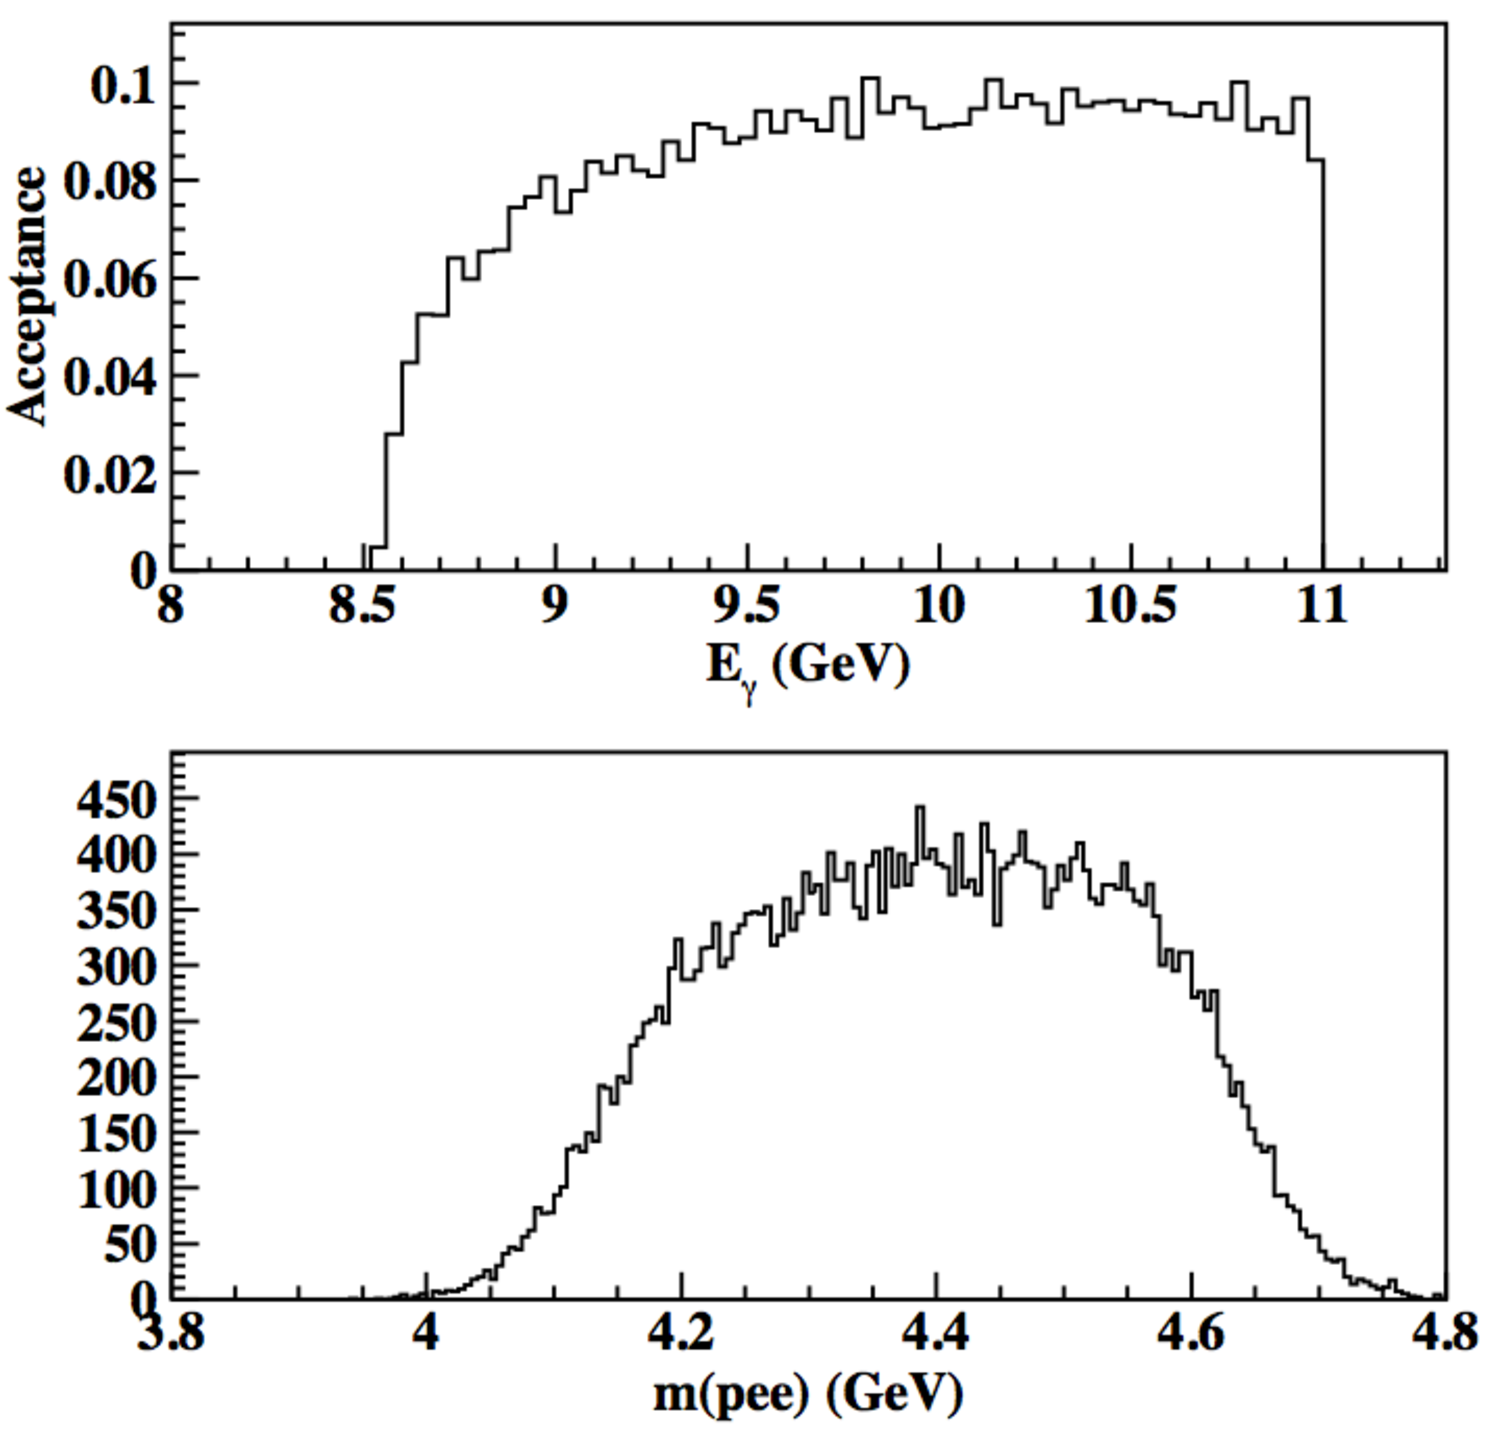
\includegraphics[width=0.9\textwidth]{pee_acceptance_mass_10.pdf}
\caption{Acceptance and the invariant mass distribution of (p$e^-e^+$) in the reaction $e p\to J/\Psi p (e^\prime)\to e^+ e^- p (e^\prime)$ for quasi-real photon energies from the threshold to 11 GeV. The smeared in Fast-MC values of momenta and angles are used to calculate the invariant mass. Minimum detection angle for particles in CLAS12-FD was set to $10^\circ$.}
\label{fig:acc_mpee_10}
\end{center}
\end{figure}
\clearpage

\section{Experiment E12-11-005}
\subsection{Introduction}

Marco: secondo me, vale subito la pena dire che questo caso ha una minor potenzialita' di scoperta ( a causa della luminosita' minore), ma in caso di segnale puo' meglio misurarne le caratteristiche (risoluzione e polarizzazione)
I due casi sono complementari! (missing e' come scoperta, e MesonEx come studio dello stato risonante)

\subsection{General features of the $\gamma^* p \rightarrow X \rightarrow J/\psi \, p$ reaction in MesonEx}

Before discussing in details the measurement $\gamma^* p \rightarrow X \rightarrow J/\psi \, p$ reaction in the MesonEx experiment, we want to briefly discuss some general features, that show the potentiality of this experiment searching for resonances decaying in the $J/\psi\, p$ final state. 

We consider the quasi-real photo-production reaction $e~p~\rightarrow~\gamma^*~p~e^{\prime}~\rightarrow~J/\psi~p~e^{\prime}$, with the final stat electron scattered at low angle and measured in the Forward Tagger detector. The final state proton and the $J/\psi$ decay products, instead, are measured in the CLAS12 detector.

In this analysis, we focused only in the $J/\psi$ decay to an electron-positron pair. We do not consider the $\mu^+ \mu^-$ decay channel, that as a comparable branching ratio, since the CLAS12 detector is not equipped with a muon identification system and, therefore, pion background would probably be too high to clearly identify the $J/\psi$ signal.


\paragraph{Invariant mass resolution: } the invariant mass $W$ of the $J/\psi\, p$ system can be measured in MesonEx as the missing mass of the final state electron, that depends only from the measured energy of the electron in Forward Tagger. Explicitly,
\begin{equation}
W^2=M_p^2+2E_0M_P-2E^{\prime}M_p \; \; ,
\end{equation}
with $E_0$, $E^{\prime}$ the primary beam energy and the final state electron energies. In particular, for $W=4449.8$ MeV (mass of the narrower $P_c$ state), $E^{\prime}=917.7$ MeV ($E^*_{\gamma}=10.08$ GeV).
Therefore, close to the mass region where resonances are expected, one has:
\begin{equation}
\sigma_W=\sigma_{E^{\prime}} \cdot \frac{M_p}{W} \simeq 0.21 \cdot \sigma_{E^{\prime}} \simeq \mbox{ 5.2 MeV}\; \; ,
\end{equation}  
being $\sigma_{E^{\prime}} \simeq$ 25 MeV the expected energy resolution for the final state electron measured in the Forward Tagger Detector \cite{Celentano:2014boa} for $E^\prime \simeq 1$ GeV. 
This value is significantly lower than the resonance width reported by LHCB for the narrower $P_c$ state, $\Gamma_a=39$ MeV, demonstrating that MesonEx is, in principle, capable of properly determining the resonance line-shape.
\paragraph{Number of measured events: } in the low $Q^{2}$ limit, the unpolarized differential reaction cross-section, with respect to the scattered electron angle $\Omega^{\prime}$ and energy $E^{\prime}$ in the laboratory frame, is \cite{Budnev:1974de}:
\begin{equation}
d\sigma(\Omega^{\prime},E^{\prime}) = \sigma_\gamma(\nu) \cdot d \Psi(\Omega^{\prime},E^{\prime}) \; \; ,
\end{equation}
with $\sigma_\gamma(\nu)$ the \textit{total} cross section for the real photo-production reaction $\gamma p \rightarrow J/\psi\, p$, being $\nu$ the virtual photon energy. The term $d \Gamma(\Omega^{\prime},E^{\prime})$ is the equivalent photon flux, given by:
\begin{equation}
d\Gamma(\Omega^{\prime},E^{\prime})=\frac{\alpha}{4\pi^{2}}\frac{E^{\prime}}{E_0}\frac{\nu}{Q^2}\left[\frac{(2E_0-\nu)^2}{\nu^2}+1  \right] d\Omega^{\prime} \,d E^{\prime}
\end{equation}
To obtain the angular-integrated photon flux, the Forward Tagger nominal acceptance has to be considered, i.e. $2.5^{\circ}<\theta^{\prime}<4.5^{\circ}$. This gives:
\begin{equation}
d\Gamma(E^{\prime})=\frac{\alpha}{4\pi}\frac{\nu}{E^2_0}\left[\frac{(2E_0-\nu)^2}{\nu^2}+1  \right] \log{ \left( \frac{1-\cos\theta_{max}}{1-\cos\theta_{min}}      \right)} d E^{\prime} \simeq 1.1 \cdot \frac{\alpha}{4\pi}\frac{\nu}{E^2_0}\left[\frac{(2E_0-\nu)^2}{\nu^2}+1  \right] d E^{\prime}
\end{equation}
To compare with the previous case (experiment E12-12-001, with the low-angle scattered electron identified in missing momentum analysis), we re-write the flux as a function of $W$:
\begin{equation}
d\Gamma(W) \simeq 1.1 \cdot \frac{\alpha}{4\pi}\frac{\nu}{E^2_0}\left[\frac{(2E_0-\nu)^2}{\nu^2}+1  \right]\frac{W}{M_p}dW
\end{equation}

At $W=4.4$ GeV, integrating over $\Delta_W=20$ MeV, this results in $\Gamma/e=1.23\cdot 10^{-5}$, an order of magnitude lower than the corresponding value in E12-12-001: 
this is a direct consequence of the lower cut-off on the $\theta^{\prime}$ angle imposed by the FT acceptance.

A reasonable estimate for the number of expected events for a resonant signal can be obtained by assuming a constant photo-production cross-section $\sigma^{\gamma}_0$, equal to the value at the resonance mass, 
and integrating in the electron energy range corresponding to the mass interval $(M-\Gamma/2,M+\Gamma/2)$, i.e. 825.1 MeV $<$ $E^{\prime}$ $<$ 1010.0 MeV for the narrower $P_c$ state ($M=4450$ MeV and $\Gamma=39$ MeV).

The foreseen rate of produced events, considering the nominal CLAS12 luminosity, $\mathcal{L}=10^{35} cm^{-2} s^{-1}$, is therefore:
 \begin{equation}
R_{gen} = \mathcal{L} \cdot \Gamma \cdot \sigma^{\gamma}_0 \simeq 2 \cdot 10^5 \cdot \sigma^{\gamma}_0 \mbox{ events / day / }\mu{\mbox barn}
\end{equation}

To get the actual number of measured events, this has to be multiplied by the branching fraction for the decay $J/\psi\rightarrow e^{+} e^{-}$ ($\simeq 5.9\%$). 
Finally, the CLAS12 acceptance $\varepsilon$ has to be considered: as discussed below, the value obtained from MonteCarlo simulations is $\varepsilon \simeq 0.13$, if all the final state particles (proton and electron-positron pair) are detected, and slightly higher if only the two leptons are measured, the proton being reconstructed via missing mass technique. This gives:
\begin{eqnarray}
R_{meas} &=& R_{gen} \cdot BR_{J/\psi\rightarrow e^{+}e^{-}} \cdot \varepsilon \simeq 1.5 \cdot 10^{3}  \cdot \sigma^{\gamma}_0 \mbox{ events / day / }\mu{\mbox barn}\\
 N_{meas} &\simeq& 1.2\cdot10^5 \cdot \sigma^{\gamma}_0 / \mu\mbox{barn} \; \; \; ,
\end{eqnarray}
considering the nominal MesonEx run time of 80 days. 

From this, a preliminary estimate of the experiment sensitivity can be derived, by requiring to have $\simeq$ 1000 events in total, i.e. $\simeq 50$ events / $W-bin$, assuming $\Delta_W=5$ MeV (the experimental resolution), and $\simeq 20$ bins 
(to properly measure the narrower $P_c$ state). The corresponding experimental sensitivity to a resonant signal is $\simeq$ 10 nbarn.


\subsection{Kinematics}
 
To simulate the measurement of the reaction $\gamma^* p \rightarrow J/\psi \, p$ with the CLAS12+Forward Tagger detector, we generated a large set of events trough a proper model, that includes two contributions:
\begin{itemize}
\item{A non-resonant production mechanism, parametrized via the $t-$channel exchange of a Pomeron trajectory. All the corresponding parameters, including the overall normalization, were tuned to reproduce the experimental data measured at higher energy  ($E_{\gamma} > 13$ GeV) \cite{Camerini:1975cy}.
We note, however, that the extrapolation of the total cross-section from the higher energy range where experimental data exist to the MesonEx range, close to the threshold, is very sensitive to the choice of the parameters. 
Specifically, with the actual values we used, we got $\sigma_{NR}(E_{\gamma}=10 \mbox{ GeV} ) = 0.2 $ nbarn \footnote
{
We observe that this value is compatible with the range predicted in \cite{bchl}, where a QCD-inspired calculation was performed.}.
} 
\item{A resonant production mechanism  , $\gamma^* p \rightarrow X \rightarrow J/\psi \, p$. 
In this note, we focused only on the narrower state reported by the LHCB experiment, $P_c(4450)$, leaving a proper study of the measurement feasibility as a function of the $X$ mass and width for the future. 
Furthermore, in the development of the production model, we only considered the $J^P$ assignment $(3/2)^-$, although we verified that this has a very limited impact on the foreseen experimental acceptance. 

This contribution is characterized by a single free parameter, the branching ratio BR of the decay $X \rightarrow J/\psi \, p$. 
The total cross section at the resonance peak reads: $\sigma_{R}(E_{\gamma}=10 \mbox{ GeV} ) = (BR)^{2}\cdot 1.3 \, \mu$barn. 
In this note, we considered the case BR $\simeq$ 0.1, so that $\sigma_{R}~\simeq~ 13$ nbarn at the resonance peak.}
\end{itemize}

The distribution of the  $J/\psi \, p$ invariant mass ($W$) is reported in Fig.~\ref{fig:1}, together with the correlation between $W$ and the momentum transferred on the proton, $-t$. 
In the production model that we developed, the $X\rightarrow J/\psi \, p$ decay is almost isotropic in the CM frame, due to the barrier-factor effects in the proximity of the $J/\psi \, p$ threshold.
 The non-resonant contribution, instead, is characterized by a diffractive-like $t$ dependence, $d\sigma / d t~\propto~\exp(- b \cdot |t|)$, with $b\simeq 2.8$ \cite{Camerini:1975cy}.

The momentum-against-angle distribution for proton and leptons, in the laboratory frame, is plotted in Fig.~\ref{fig:2}. 
The proton is always emitted at low angle, $\theta_P < 25^{\circ}$, due to the lower mass with respect to the $J/\psi$ meson. 
The $e^{+}$ and the $e^{-}$, instead, are typically emitted at larger angle, with a significant fraction of events with one or both out of the CLAS12-FD acceptance.
\begin{figure}[tpb]
\subfigure{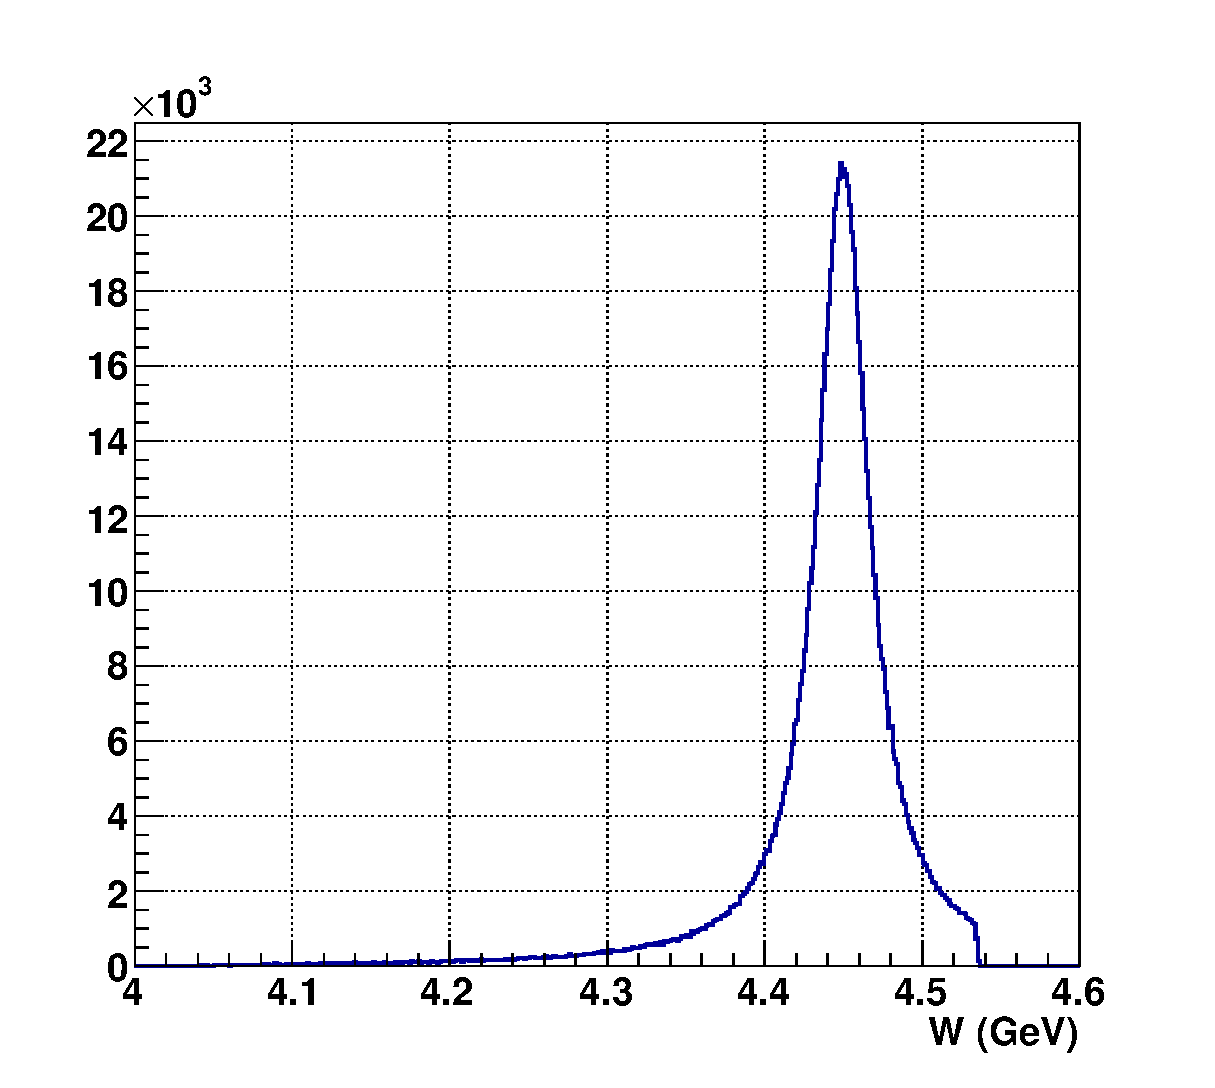
\includegraphics[width=0.45\textwidth]{WGEN.eps}}
\subfigure{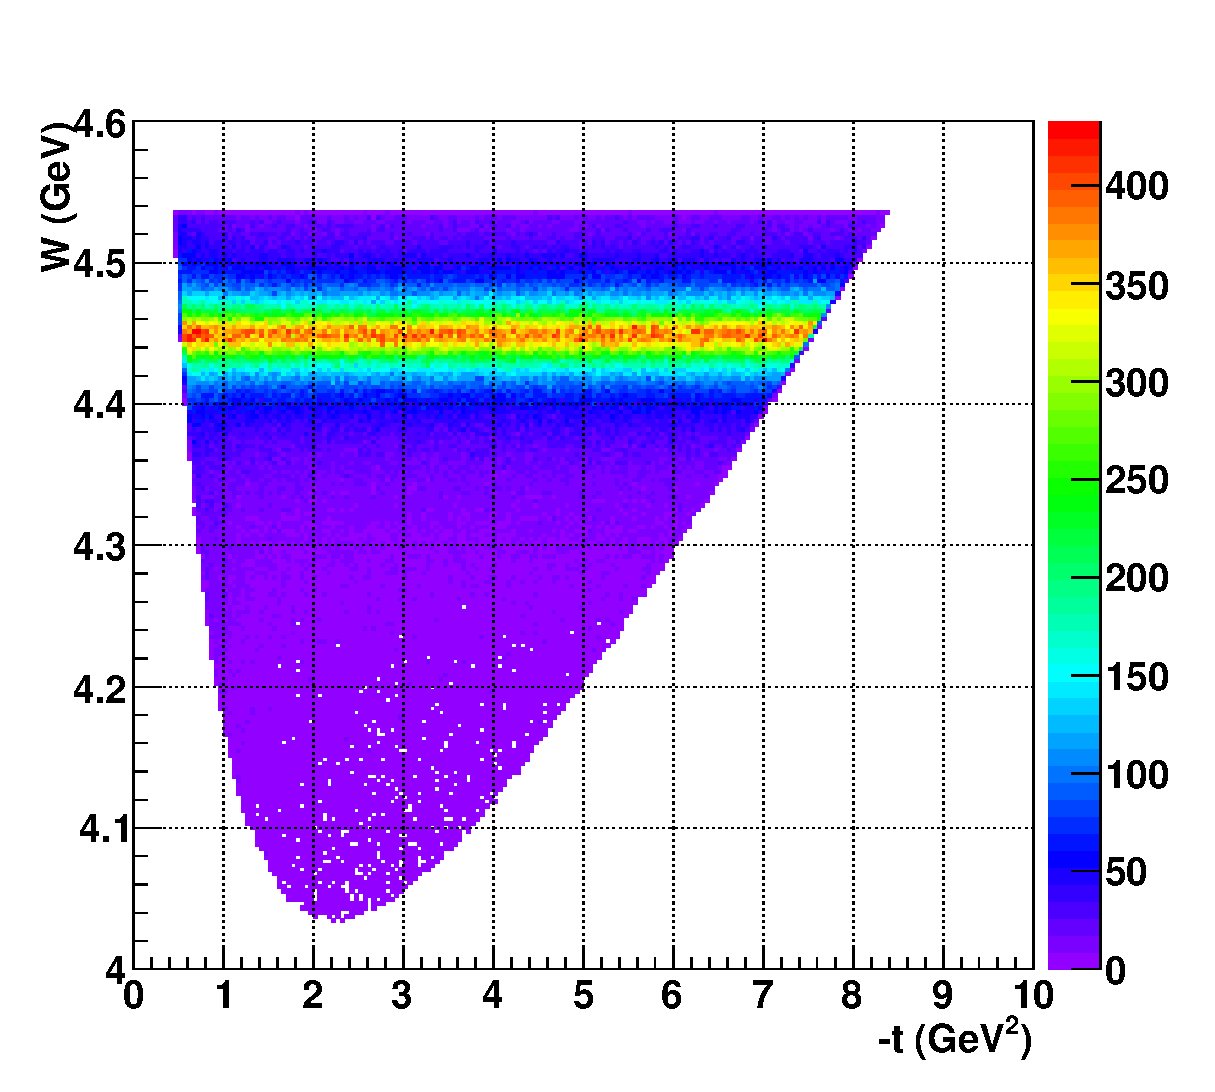
\includegraphics[width=0.45\textwidth]{WvstGEN.eps}}
\caption{\footnotesize \label{fig:1} Left: $J/\psi \, p$ invariant mass distribution. Right: $J/\psi \, p$ invariant mass vs momentum transfer on the proton distribution.}
\end{figure}

\begin{figure}[tpb]
\subfigure{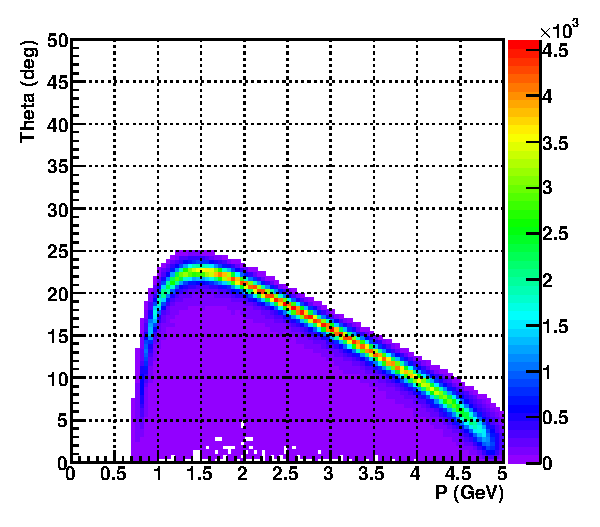
\includegraphics[width=0.45\textwidth]{protonGEN.eps}}
\subfigure{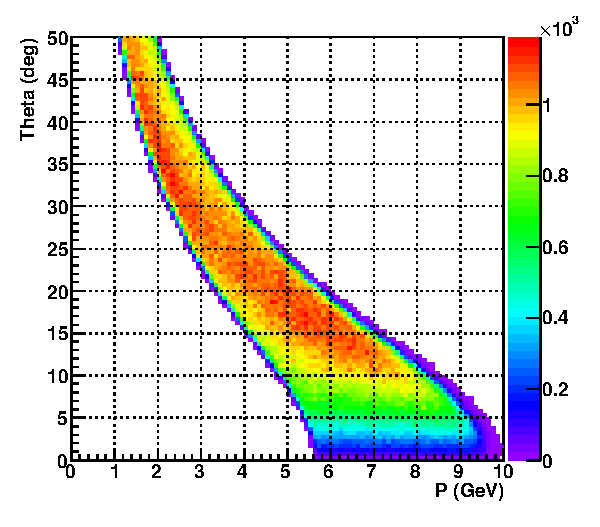
\includegraphics[width=0.45\textwidth]{leptonGEN.eps}}
\caption{\footnotesize \label{fig:2} Momentum-against-angle distribution for the final state proton (left) and for the leptons (right), in the laboratory frame.}
\end{figure}




\subsection{Detector response}

The reaction that we consider foresees 4 particles in the final state: a low-angle scattered electron, measured with the Forward Tagger facility, and a proton and an electron-positron pair from $J/\psi$ decay, measured with the CLAS12 detector. Since the CLAS12-Central Detector (CD) is not suited for electron detection and identification, we consider only the detection of final state leptons in the CLAS12-Forward Detector (FD). Two possible measurement strategies are possible:
\begin{itemize}
\item{Measure \textit{all} the final state particles, reconstructing the $J/\psi$ via the invariant mass of the electron-positron pair.}
\item{Measure \textit{only} the scattered electron in the Forward Tagger and the electron-positron pair in CLAS12-FD, reconstructing the $J/\psi$ via the invariant mass of the $e^{+} e^{-}$ system and the proton via the missing mass on it.}
\end{itemize} 
While the first solution would permit a better background discrimination, given the larger control on kinematics variable that the full measure of the final state permits, the second results in a slightly larger experimental acceptance. A proper discussion on the best measurement strategy would require a full simulation of the backgrounds associated with the measurement, not performed in this note: for this reason, in the following we will discuss both strategies. 

The CLAS12 and Forward Tagger response was simulated using the Fast MonteCarlo (FASTMC) software, that effectively accounts for the detector geometrical acceptance and resolution. Each final state particle, i.e. the recoil
proton, the scattered electron, and the two leptons, is projected individually on the detector. If it is within the nominal detector acceptance region, the four-momentum is smeared according to the expected resolution, otherwise it is discarded. We made the following conservative assumptions:
\begin{itemize}
\item{The CLAS12-CD acceptance for leptons is zero. As discussed, this reflects the fact that this detector is not designed for $e^- / e^+$ detection and identification.}
\item{We considered only events with both the electron and the positron from $J/\psi$ decay detected in the CLAS12-CD, i.e. we neglected the possibility that they are measured with the Forward Tagger.}
\end{itemize}

The resolution on the reconstructed $J/\psi$ mass, from the $e^{+} e^{-}$ measured four vectors, is reported in Fig.~\ref{fig:3}. At the maximum value of the CLAS12 toroidal field, with positive (negative) particles being outbended (inbeded), a resolution of $\simeq 15$ MeV is obtained, as shown in the left panel. The right panel, instead, reports the resolution on the $e^- - e^+$ missing mass, relevant for the second measurement strategy outlined before.

\begin{figure}[tpb]
\subfigure{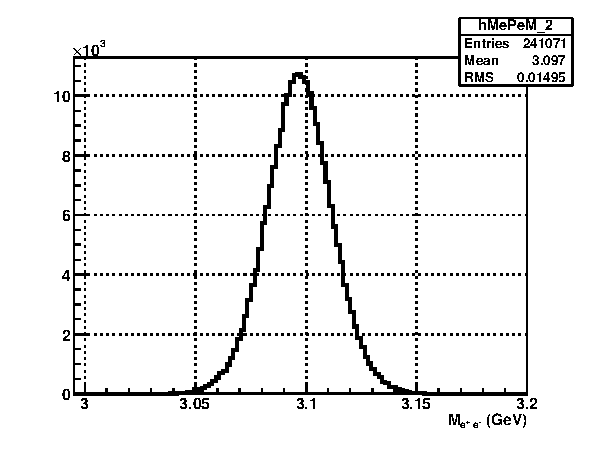
\includegraphics[width=0.45\textwidth]{resJPSInominal.eps}}
\subfigure{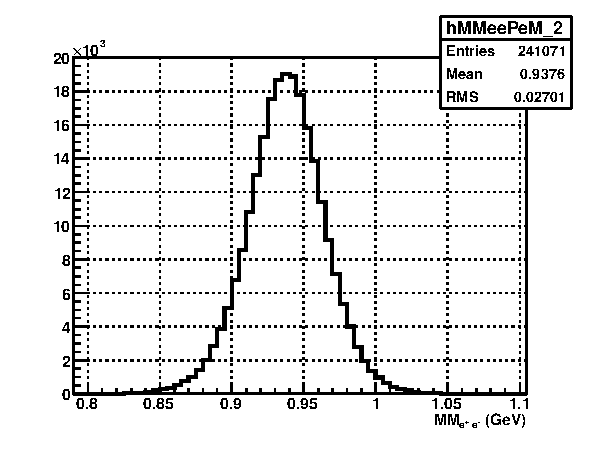
\includegraphics[width=0.45\textwidth]{resPnominal.eps}}
\caption{\footnotesize \label{fig:3} Left: reconstructed $J/\psi$ mass. Right: missing mass on the $e^+\,e^-$ pair. Both plots refer to the maximum value of the CLAS12 toroidal field, configured to have positive particles outbending.}
\end{figure}

We also investigated the effect of a magnetic field variation on the above quantities. As expected, we observed that there is almost no dependence on the orientation of the CLAS12 toroidal field, given the charge symmetry of the $e^+ e^-$ system. Results are reported in Fig.~\ref{fig:4}.

\begin{figure}[tpb]
\subfigure{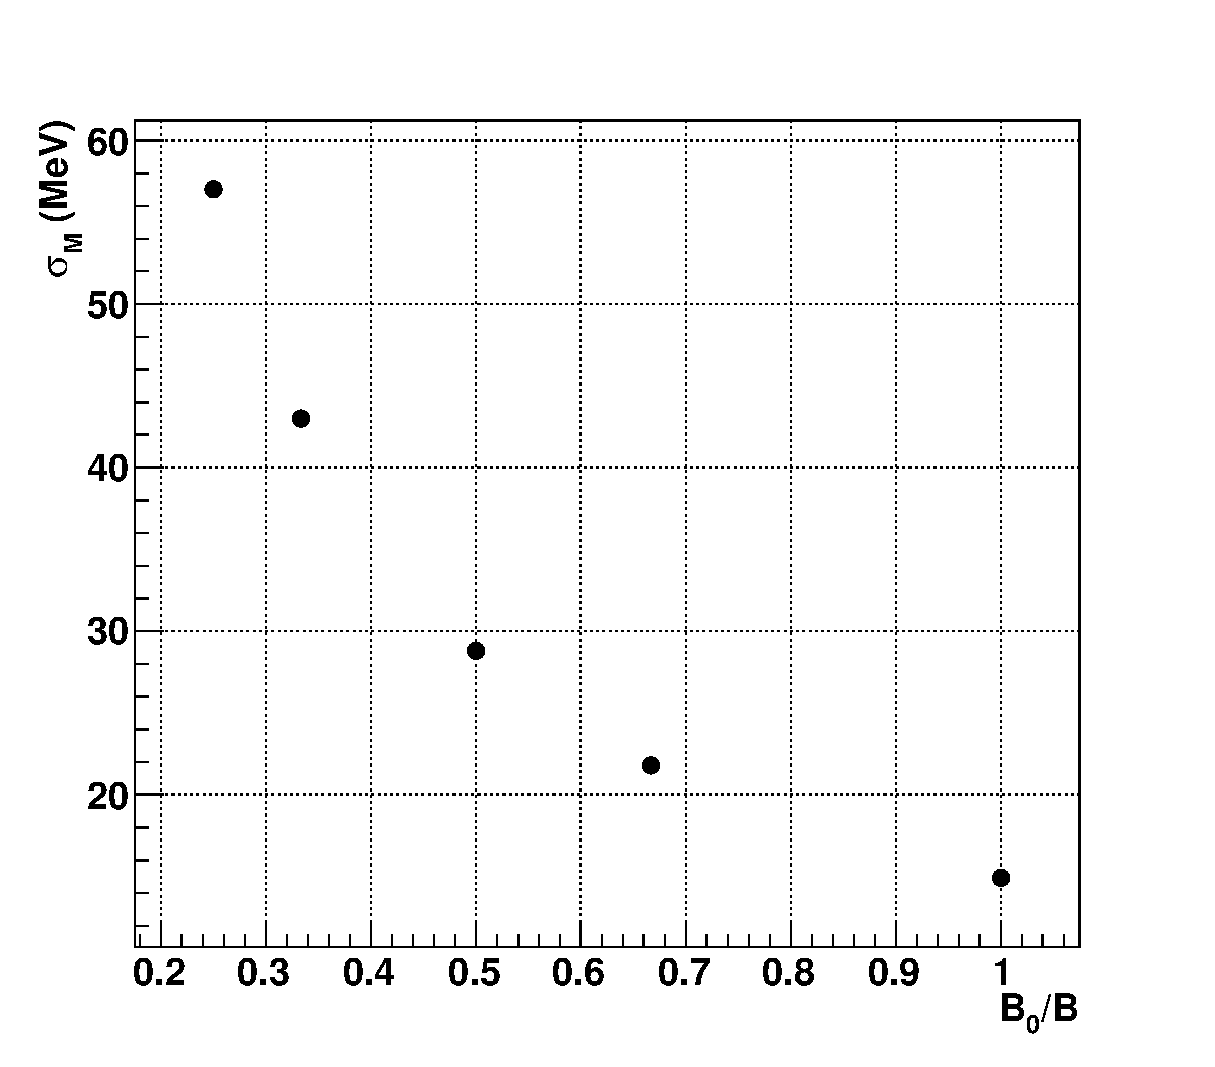
\includegraphics[width=0.45\textwidth]{resJPSIfield.eps}}
\subfigure{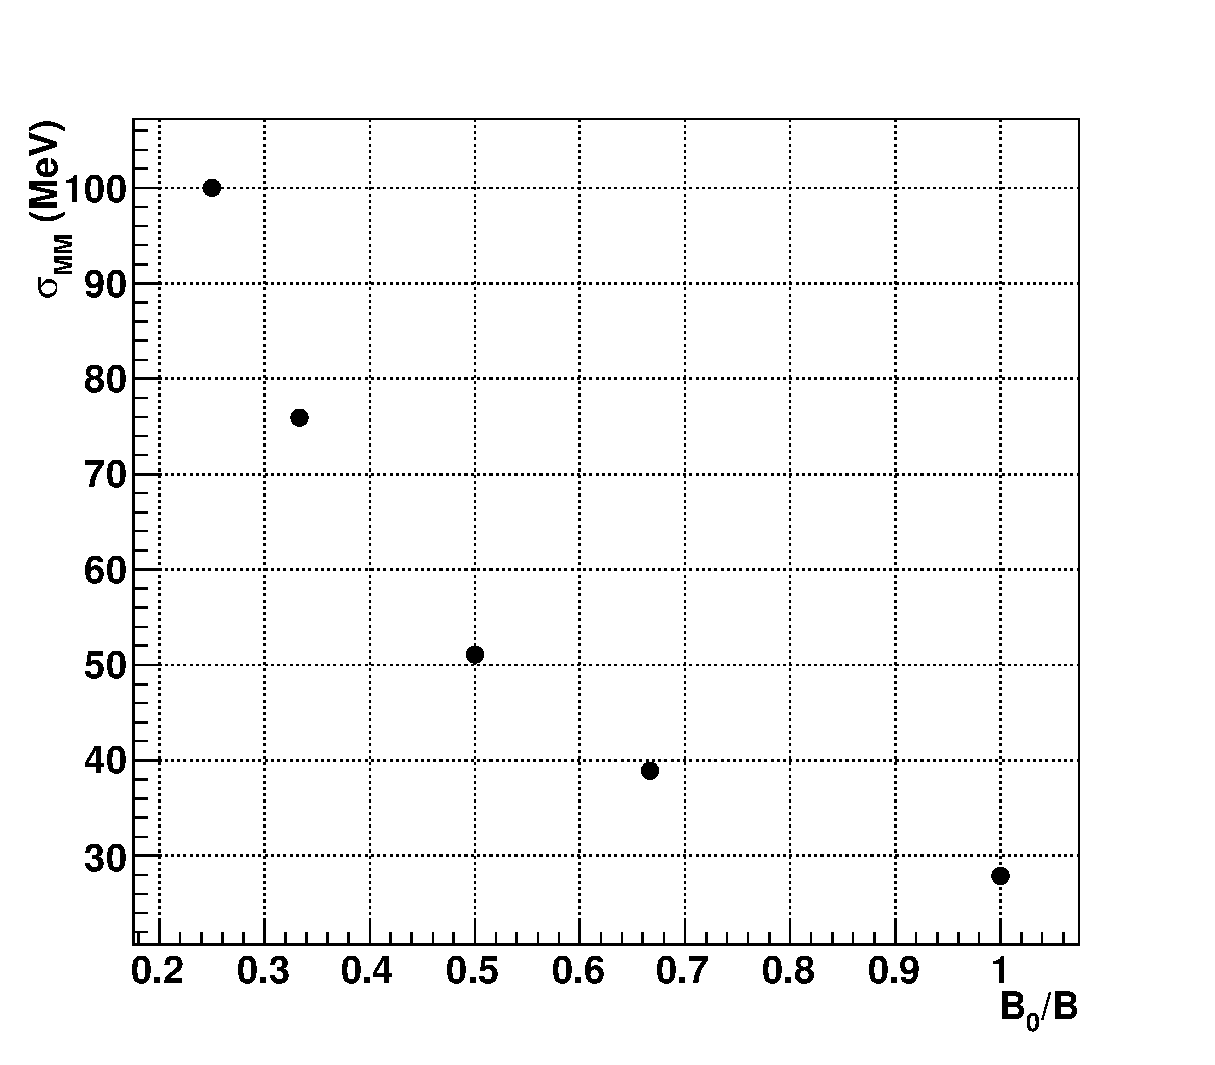
\includegraphics[width=0.45\textwidth]{resPfield.eps}}
\caption{\footnotesize \label{fig:4} Left: reconstructed $J/\psi$ mass resolution as a function of the CLAS12 toroidal field intensity (normalized to the maximum possible value). Right: resolution on the missing mass on the $e^+\,e^-$ pair as a function of the CLAS12 toroidal field intensity.}
\end{figure}

The CLAS12 acceptance, as a function of the $J/\psi\, p$ invariant mass $W$, is reported in Fig.~\ref{fig:5}, for both measurement strategies outlined below. For both cases, the acceptance shows a smooth increase with $W$, with an average value of $\simeq 13\%$ for the detection of all final state particles ($\simeq 16\%$ for the detection of the $e^{+} e^{-}$ pair only). We observe that the ``deep'' at $W=4.4$ GeV, at the resonance mass, is due to the fact that resonance production mechanism is characterized by a very different kinematics than the background, in particular for the $t$ dependence, and, therefore, the corresponding CLAS12 response is different. 

We also investigated the effect of a change in the CLAS12 toroidal field, finding a very modest dependence on in. 
The larger effect comes from inverting the polarity of the field, i.e. having the proton being inbended by the field. In this case, the acceptance for the measure of all the final state particles drops to $\simeq 9\%$, while there is no change for the measure of the $e^+ e^-$ pair only.

\begin{figure}[tpb]
\center
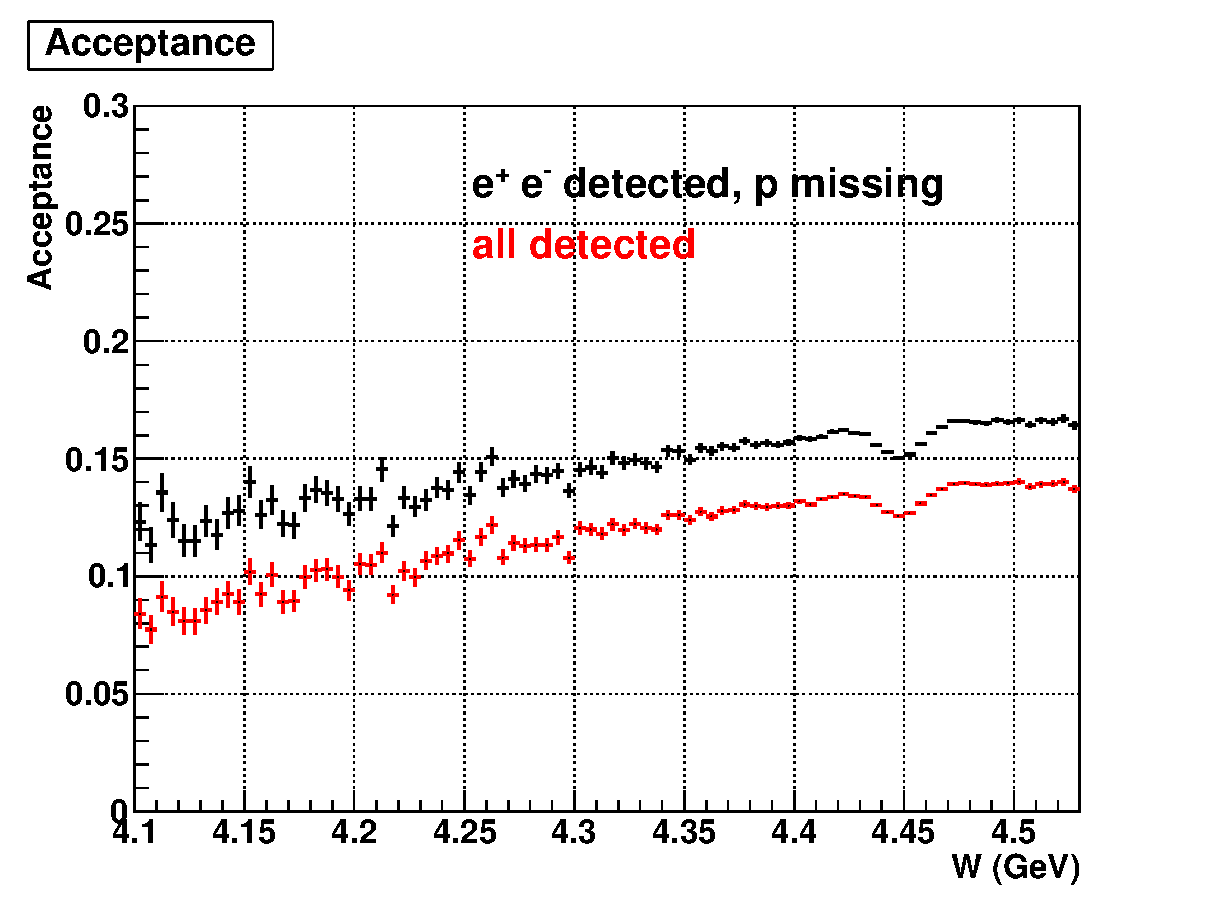
\includegraphics[width=0.7\textwidth]{acceptanceNominal.eps}
\caption{\footnotesize \label{fig:5} Detector acceptance as a function of the  $J/\psi\, p$ invariant mass, for both measurement strategies outlined before. Both plots refer to the maximum value of the CLAS12 toroidal field, configured to have positive particles outbending. }
\end{figure}

Finally, the resolution on the $J/\psi\, p$ invariant mass $W$, \textit{measured as the missing mass on the low-angle scattered electron}, is shown in Fig.~\ref{fig:6}. As pointed before, this quantity depends only on the measurement of the final state electron with the Forward Tagger calorimeter, and it is almost insensitive to the CLAS12 configuration. For $W=4.4$ GeV, $\sigma_W=5.5$ MeV, in agreement with the previous estimate.

\begin{figure}[tpb]
\center
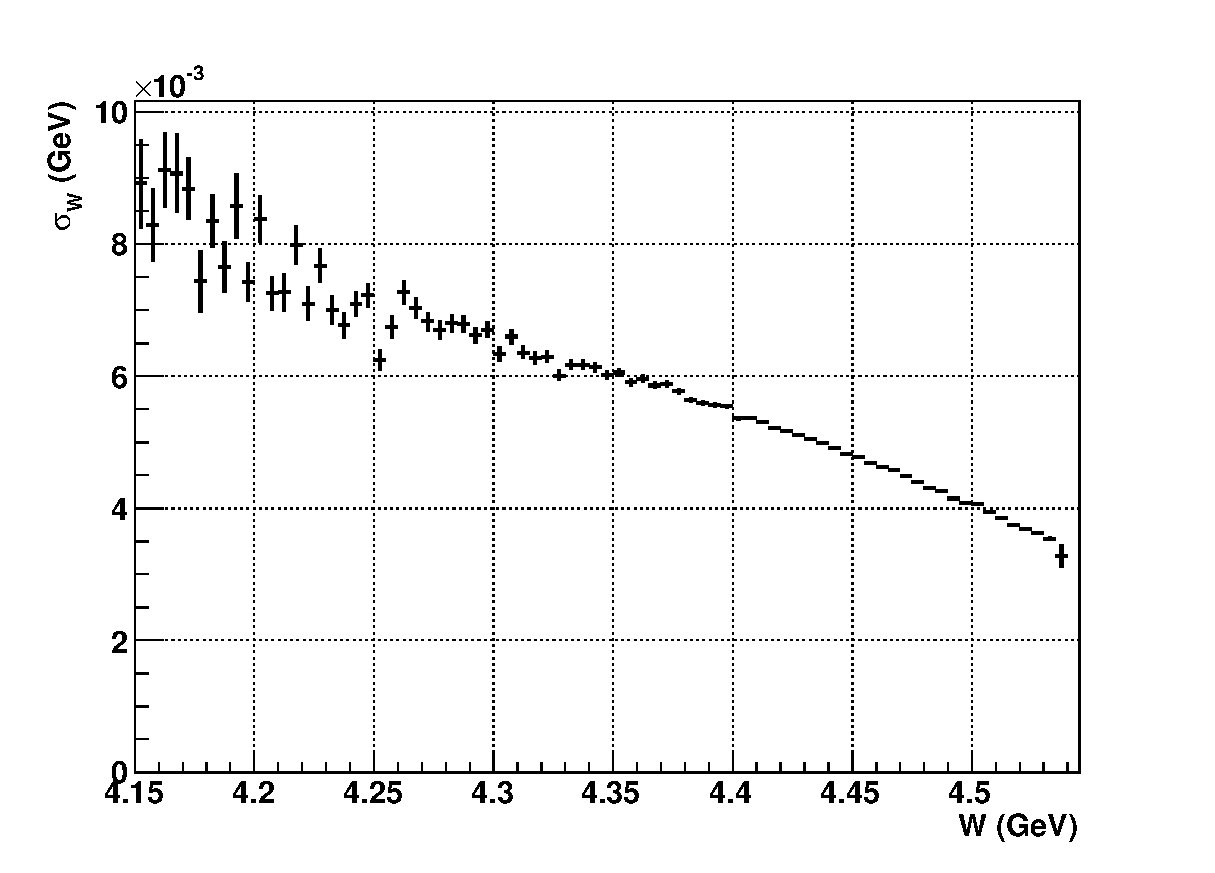
\includegraphics[width=0.7\textwidth]{resolutionW.eps}
\caption{\footnotesize \label{fig:6} Resolution on the  $J/\psi\, p$ invariant mass.}
\end{figure}











\section{J/$\Psi$ electroprodustion experiment}

There an ideate study Double-DVCS and the \JP electroproduction using modified CLAS12 detector \cite{dimuon_loi}. The modification to CLAS12 is quite simple, there will be iron absorber/shield instead of High Threshold Cherenkov Counter part of which will lead-tungsten calorimeter. The shield/absorber will play double role, it will be hadron filter for muon detector, which is the CLAS12 forward detector, and will be a shield for forward drift chambers to allow for high luminosity running. The proposed experiment will study reaction  $e p\to e^\prime J/\Psi p \to e^\prime\mu^+ \mu^- (p)$ in a wide range of kinematics. In these final states, the pentaquarks will be searched in the missing mass of the scattered electron, $e^\prime$. It is expected energy resolution of the calorimeter to be on order of $\sim 3.5\%/\sqrt E$. The missing mass resolution will not be great and will be a problem for the narrow pentaquark searches. The mass resolution will be similar to the expected resolution for E12-11-005. 

The experiment is expected to run at $\times 50$ to $\times 100$ above the CLAS12 nominal luminosity, still due to the large scattering angle of the primary electron (large Q$^2$) rates will be  small. But, if pentaquark resonances exist and the photoproduction cross sections are close to what have been predicted in literature, this will be the first experiment to study pentaquarks in electroproduction.     

\section{Summary}

There is a viable option for searches of LHCb hidden charmed pentaquarks, $P_c(4380)$ and $P_c(4450)$, in the photoproduction reaction using the CLAS12 detector in Hall-B and the 11 GeV electron beam. Experiments E12-11-005 \cite{e1211005} and E12-12-001 \cite{e1212001}, and the new proposal for electroproduction of J/$\Psi$ are well suited to search and study charmed pentaquarks with electromagnetic probs. Options for higher than the nominal luminosity running for these experiments must be studied with GEANT simulations to estimate the background and limitations. 

\begin{thebibliography}{99}

\bibitem{lhcb_penta}The LHCb Collaboration, http://arxiv.org/pdf/1507.03414v2.pdf
\bibitem{e1211005} M. Battaglieri et al., https://www.jlab.org/exp\_prog/proposals/12/PR12-11-0015.pdf
\bibitem{e1212001} S. Stepanyan et al., https://www.jlab.org/exp\_prog/proposals/12/PR12-12-001.pdf
\bibitem{pt1}Q. Wang, X.-H. Liu, and Q. Zhao, http://arxiv.org/abs/1508.00339v1
\bibitem{pt2} V. Kubarovsky and M.B. Voloshin, http://arxiv.org/abs/1508.00888v1
\bibitem{pt3} M. Karlineray and J. L. Rosner, http://arxiv.org/abs/1508.01496v1
\bibitem{pt4} V. Kubarovsky, will be published as a note.
\bibitem{tcs_rafo}R. Paremuzyan, https://www.jlab.org/Hall-B/general/thesis/Paremuzyan\_thesis.pdf
\bibitem{jpc_prop}I. Aznauryan et al., https://www.jlab.org/exp\_prog/proposals/07/PR-07-009.pdf
\bibitem{bchl} S.J. Brodsky. E. Chudakov, P. Hoyer, J.M. Laget, http://arxiv.org/pdf/0010343 (2000).
\bibitem{Phot_Flux1} \url{ http://lss.fnal.gov/archive/other/lpc-94-35.pdf}
%MesonEx biblio starts here
\bibitem{Celentano:2014boa} A.~Celentano [CLAS Collaboration], EPJ Web Conf.\  {\bf 73}, 08004 (2014).
\bibitem{Budnev:1974de} V.~M.~Budnev, I.~F.~Ginzburg, G.~V.~Meledin and V.~G.~Serbo, Phys.\ Rept.\  {\bf 15}, 181 (1975).
\bibitem{Camerini:1975cy} U.~Camerini {\it et al.},  Phys.\ Rev.\ Lett.\  {\bf 35}, 483 (1975).

%MesonEx biblio ends here
\bibitem{PDG} Chin. Phys. C, 38, 090001 (2014)
\bibitem{dimuon_loi} S. Stepanyan et al., https://userweb.jlab.org/~stepanya/clas12/dileptons/dimuons\_clas12.pdf

\end{thebibliography}

\end{document}
